\newpage
\chapter{Resultados}
\addcontentsline{toc}{chapter}{Resultados}
% Automatically generated. Do not edit.
\newcommand{\LinkCount}{1.310 }
\newcommand{\ConstantSimilarityCutoff}{0,72}


Nesta seção são apresentados os resultados obtidos nas principais etapas do
estudo: coleta das comunicações públicas do Federal Reserve, preparação dos
textos, extração e classificação dos sinais de política monetária por modelos
de linguagem, construção da rede de similaridade semântica, 
definição do indicador e validação da sua capacidade de refletir a orientação 
da política monetária.

Além de descrever o conjunto de dados e os sinais identificados, são analisadas
as propriedades da rede construída, incluindo a distribuição das conexões, a
formação de comunidades e a relevância estrutural dos nós. Por fim, os resultados
são organizados temporalmente para avaliar a relação entre a orientação dos sinais
extraídos e as decisões observadas do Federal Open Market Committee (FOMC).

\section{Coleta dos links das publicações}

Na etapa inicial da pesquisa, foram coletados, usando Python, os links referentes às comunicações
públicas disponibilizadas pelo Federal Reserve em seu site oficial. Ao todo, foram
obtidos \LinkCount links. O objetivo
foi estruturar as origens da base documental à ser utilizada nas etapas de extração textual e 
classificação dos sinais de política monetária.

Foram consideradas páginas relacionadas aos materiais de política monetária, ao
calendário do Federal Open Market Committee (FOMC) e às comunicações públicas de
dirigentes, como discursos e testemunhos. Os endereços apresentados na
Tabela~\ref{tab:fontes-coleta} correspondem a páginas institucionais de consulta
que reúnem links para os textos integrais das publicações, e não aos documentos
individuais que compõem a base. Em particular, o Calendário do FOMC disponibiliza
os links para as atas e os comunicados associados a cada reunião do Comitê. A partir
dessas páginas, foram extraídos os links das comunicações publicadas entre janeiro
de 2015 e setembro de 2025. 

\begin{table}[htb]
\caption{Páginas do Federal Reserve utilizadas como fontes iniciais para a coleta.}
\label{tab:fontes-coleta}
\begin{tabular}{p{0.38\textwidth} p{0.52\textwidth}}
\hline
\textbf{Fonte consultada} & \textbf{Endereço eletrônico} \\
\hline
Materiais de política monetária &
https://www.federalreserve.gov/ \newline{monetarypolicy/materials/} \\
\hline
Calendário do FOMC &
https://www.federalreserve.gov/ \newline{monetarypolicy/fomccalendars.htm} \\
\hline
Discursos e testemunhos &
https://www.federalreserve.gov/ \newline{newsevents/speeches-testimony.htm} \\
\hline
\end{tabular}
\\
\makebox[\textwidth][l]{Fonte: Autoria própria.}
\end{table}

O procedimento de coleta dos links combinou ferramentas distintas de acordo com a estrutura
de cada página. Para os materiais de política monetária e para as páginas de
discursos e testemunhos, que houve necessidade de navegação paginada,
foi utilizado a biblioteca Selenium com o navegador Microsoft Edge. Essa ferramenta permitiu
carregar as páginas, avançar entre os resultados e identificar os elementos HTML
que continham os links das publicações. Já no calendário do FOMC, foram realizadas
requisições HTTP com a biblioteca Requests, seguidas da análise do código HTML com
Beautiful Soup. 

\section{Extração e padronização dos textos}

Após a obtenção dos endereços eletrônicos das publicações, foi realizada a 
etapa de extração e padronização de seu conteúdo textual. Os resultados foram 
armazenados em formato JSON, mantendo-se, para cada publicação processada, 
a URL de origem, o título, a data de publicação e o texto extraído. 
Antes do processamento de um novo endereço, eram verificadas as URLs 
já presentes no conjunto de dados, evitando o processamento repetido de 
publicações previamente extraídas.

Para as publicações disponibilizadas diretamente em páginas HTML, foram realizadas 
requisições HTTP por meio da biblioteca \textit{Requests}. As requisições foram 
configuradas com tempo limite de resposta e, após o recebimento do conteúdo, 
sua codificação foi definida como UTF-8. O documento HTML retornado foi então 
interpretado utilizando a biblioteca \textit{Beautiful Soup}.

Antes da obtenção do texto, foram removidos elementos HTML sem 
interesse para a análise, especificamente as tags \texttt{script}, 
\texttt{style}, \texttt{noscript}, \texttt{header}, \texttt{footer} e 
\texttt{nav}. Em seguida, o conteúdo restante da página foi convertido em 
texto, utilizando quebras de linha como separadores. Cada linha foi 
posteriormente tratada para remoção de espaços excedentes em suas extremidades, 
e as linhas vazias foram descartadas. O resultado desse procedimento constituiu 
o conteúdo textual utilizado nas etapas seguintes do trabalho.

A identificação do título e da data de publicação foi realizada com auxílio 
de um modelo de linguagem de grande escala. O texto obtido após o tratamento 
da página HTML foi fornecido ao modelo juntamente com uma instrução para 
retornar essas duas informações em formato JSON. A data de publicação 
foi padronizada no formato \texttt{YYYY-MM-DD}. Após o processamento, 
a URL original e o conteúdo textual previamente extraído eram incorporados 
ao registro, resultando em uma estrutura padronizada para cada publicação.

Para documentos cujo conteúdo estava disponibilizado em arquivos PDF, 
foi adotado um procedimento específico. Inicialmente, a página associada à 
publicação era obtida por meio de uma requisição HTTP e 
processada com \textit{Beautiful Soup}. Todas as tags de 
hiperlink \texttt{<a>} eram examinadas e seus atributos \texttt{href} avaliados 
para identificar endereços contendo a extensão \texttt{.pdf}.

Após a identificação do arquivo, uma nova requisição HTTP era realizada 
para seu download. O documento era armazenado temporariamente como arquivo 
PDF e processado com a biblioteca \textit{PyPDF2}. A extração era realizada 
sequencialmente, percorrendo todas as páginas do documento por meio 
da classe \texttt{PdfReader} e concatenando o conteúdo textual obtido. 
Após a conclusão da leitura, o arquivo temporário era removido.

Durante a preparação, os documentos cujo título continha a expressão
\textit{implementation note} foram marcados como não extraídos, em vez de terem seu
conteúdo utilizado nas etapas seguintes. Ao final de cada processamento, o registro
era acrescentado ao arquivo JSON, que era atualizado incrementalmente. Esse
procedimento permitiu preservar os dados já coletados e retomar a execução sem
duplicar publicações.

Como resultado da etapa de extração, cada comunicação passou a ser representada
em uma estrutura padronizada, contendo quatro campos principais: 
\texttt{url}, \texttt{title}, \texttt{text} e \texttt{publication\_date}, 
conforme ilustrado
na Figura~\ref{fig:resultado-extracao-texto}.

\begin{figure}[htb]
	\centering
	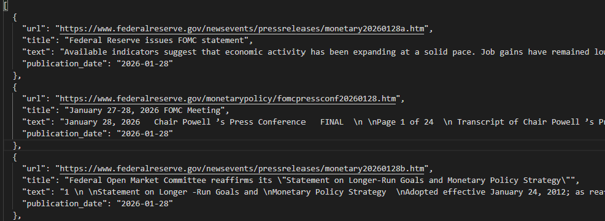
\includegraphics[width=\textwidth]{figuras/resultado_extracao_texto.png}
	\caption{Exemplo da estrutura JSON produzida na etapa de extração dos textos. 
  \newline Fonte: Autoria própria.}
	\label{fig:resultado-extracao-texto}

\end{figure}


\section{Extração e classificação dos sinais monetários}

Após a estruturação da base textual, foi realizada a etapa de identificação e 
classificação dos sinais de política monetária presentes nas comunicações do 
Federal Reserve. Para essa finalidade, foi utilizado um modelo de linguagem de 
grande porte, instruído por meio de um prompt estruturado a atuar como um 
economista especializado na análise de comunicações de bancos centrais e de 
sinais relacionados à política monetária.

Para cada documento, o prompt recebeu como contexto três informações 
provenientes da etapa anterior: o título da publicação, a data de 
publicação e o conteúdo textual da comunicação. A partir dessas 
informações, o modelo \texttt{gpt-5.6-terra} foi instruído a identificar 
somente sinais relacionados à política monetária e a classificar 
cada sinal de acordo com a orientação monetária implícita. A execução 
foi configurada para produzir respostas estruturadas em formato JSON, 
com temperatura igual a zero e sem esforço adicional de raciocínio.

Foram definidas cinco categorias de orientação monetária: 
\textit{dovish}, \textit{mostly dovish}, \textit{neutral}, 
\textit{mostly hawkish} e \textit{hawkish}. As definições 
incorporadas ao prompt consideraram principalmente informações 
relacionadas à inflação, à atividade econômica, ao mercado de 
trabalho e à orientação esperada da política monetária. 
Os critérios utilizados são apresentados na Tabela~\ref{tab:classes-sinais}.

\begin{table}[H]
\centering
\caption{Descrição das classes para classificação dos sinais monetários.}
\label{tab:classes-sinais}
\begin{tabular}{p{0.20\textwidth} p{0.70\textwidth}}
\hline
\textbf{Classe} & \textbf{Descrição} \\
\hline
\textit{dovish} & Clearly supports monetary easing or maintaining an 
accommodative stance. Use when the signal indicates that inflation is 
at target, below target, or moving sustainably toward target; economic 
activity is weakening; or labor market conditions are softening in a 
way that reduces the need for restrictive policy. \\
\hline
\textit{mostly dovish} & Leans toward monetary easing or delaying 
further tightening, but it is not definitive. Use when the signal 
reports progress on inflation, slower growth, or softer labor market 
conditions, while also mentioning uncertainty. \\
\hline
\textit{neutral} & The signal does not clearly imply either easing 
or tightening. Use when it does not indicate a dominant direction 
for policy. Do not classify as neutral merely because it is factual 
or descriptive. \\
\hline
\textit{mostly hawkish} & Leans toward monetary tightening or 
delaying easing, but it is not definitive. Use when the signal 
reports elevated inflation, upside inflation risks, resilient demand, 
or strong labor market conditions, while also mentioning uncertainty. \\
\hline
\textit{hawkish} & Clearly supports monetary tightening or 
maintaining a restrictive stance. Use when the signal indicates 
that inflation is above target, persistent, broad-based, or rising; 
economic activity remains strong; or labor market conditions remain 
tight in a way that justifies restrictive policy. \\
\hline
\end{tabular}
\\
\makebox[\textwidth][l]{Fonte: Autoria própria.}
\end{table}


Além das definições das classes, o prompt estabeleceu regras para 
tornar a extração mais consistente. Foram considerados apenas sinais 
relacionados à política monetária, e cada sinal deveria representar uma 
única ideia principal. Para cada classificação, o modelo deveria retornar 
uma lista de sinais identificados, sendo utilizada uma lista vazia 
quando nenhum sinal correspondente fosse encontrado no documento.

A saída esperada foi definida como um objeto JSON organizado pelas 
cinco categorias de classificação. Para cada sinal identificado, 
foram retornados três campos:

\begin{itemize}
\item \textit{signal}: síntese da principal informação ou sinal de 
política monetária identificado;
\item \textit{justification}: breve justificativa para a 
classificação atribuída;
\item \textit{evidence}: trecho curto, reproduzido diretamente da 
comunicação original, utilizado como evidência para o sinal identificado.
\end{itemize}

O prompt completo utilizado nessa etapa é apresentado no 
Apêndice~\ref{ap:prompt-extracao}.


Na próxima etapa, cada sinal foi convertido em um registro individual. 
A classificação textual foi então associada a um escore numérico por 
meio de um mapeamento determinístico, independente do modelo de linguagem. 
Os valores variam de $-1$, correspondente à orientação mais \textit{dovish}, 
a $1$, correspondente à orientação mais \textit{hawkish}, conforme apresentado na
Tabela~\ref{tab:score-sinais}.

\begin{table}[htb]
\centering
\caption{Mapa da classificação para o escore.}
\label{tab:score-sinais}
\begin{tabular}{p{0.45\textwidth} p{0.20\textwidth}}
\hline
\textbf{Classificação} & \textbf{Escore} \\
\hline
\textit{dovish} & -1 \\
\textit{mostly\_dovish} & -0,5 \\
\textit{neutral} & 0 \\
\textit{mostly\_hawkish} & 0,5 \\
\textit{hawkish} & 1 \\
\hline
\end{tabular}
\\
\makebox[\textwidth][l]{Fonte: Autoria própria.}
\end{table}

Além da classificação e do escore, foi gerada uma representação vetorial 
para cada sinal extraído. Para isso, somente o conteúdo do campo 
\texttt{signal} foi fornecido ao modelo de embeddings \texttt{text-embedding-3-large}. 
Cada sinal foi representado por um vetor com 3.072 componentes, 
armazenado no campo \texttt{embedding\_signal}. Esses vetores foram posteriormente 
utilizados para representar a proximidade semântica entre os sinais 
monetários e constituir as relações de similaridade empregadas na construção do grafo.

Ao final do processamento, cada sinal monetário passou a corresponder 
a uma linha da base tabular, contendo os campos 
\texttt{url}, \texttt{title}, \texttt{publication\_date}, 
\texttt{classification}, \texttt{score}, \texttt{signal}, 
\texttt{justification}, \texttt{evidence} e \texttt{embedding\_signal}. 
Os novos registros eram concatenados aos resultados já existentes e 
armazenados incrementalmente em arquivo CSV, permitindo preservar os 
sinais previamente processados e retomar a execução sem duplicação de documentos.

\section{Construção do grafo}

Após a estruturação e classificação dos sinais monetários, os dados foram 
inseridos em um banco de dados orientado a grafos utilizando o Neo4j. 
A modelagem adotada foi composta por dois tipos de nós: 
\texttt{Publication}, utilizado para representar cada comunicação do 
Federal Reserve, e \texttt{Signal}, utilizado para representar 
individualmente os sinais de política monetária extraídos dessas comunicações.

Os nós \texttt{Publication} foram identificados de forma única pela 
URL da publicação. Para cada nó, foram armazenadas as 
propriedades \texttt{title} e \texttt{publication\_date}, correspondentes, 
respectivamente, ao título e à data de publicação do documento. 
O uso da URL como identificador permitiu que diferentes sinais extraídos 
de uma mesma comunicação fossem associados a um único nó de publicação.

Os nós \texttt{Signal}, por sua vez, foram identificados pela 
combinação entre o conteúdo textual do sinal e a URL da publicação 
de origem. Dessa forma, sinais com conteúdos semelhantes ou mesmo 
idênticos, mas provenientes de documentos distintos, puderam ser 
mantidos como entidades independentes no grafo. 
Cada nó recebeu as propriedades \texttt{classification}, 
\texttt{score}, \texttt{justification}, \texttt{evidence}, 
\texttt{embedding\_signal} e \texttt{date}. A propriedade 
\texttt{date} corresponde à data de publicação do documento 
do qual o sinal foi extraído.

A vinculação entre as publicações e os sinais foi representada 
pela relação \texttt{HAS\_SIGNAL}, criada entre cada 
nó \texttt{Publication} e os respectivos nós \texttt{Signal}. 
Essa estrutura preserva a origem documental de cada sinal e, 
em conjunto com as propriedades \texttt{justification} e 
\texttt{evidence}, permite rastrear a classificação até o 
conteúdo da comunicação utilizada pelo modelo de linguagem.

Além das relações entre publicações e sinais, foram construídas 
relações \texttt{SIMILAR\_TO} entre sinais semanticamente próximos. 
Essas conexões foram obtidas a partir da comparação dos vetores 
armazenados em \texttt{embedding\_signal} e receberam a propriedade 
\texttt{score\_similarity}, correspondente à similaridade entre os 
respectivos vetores. Como a proximidade semântica representa uma 
associação simétrica, a direção das relações foi desconsiderada 
nas projeções utilizadas nas análises de rede.

Diferentemente dos nós e das relações \texttt{HAS\_SIGNAL}, 
que constituem a estrutura permanente do grafo, as relações 
\texttt{SIMILAR\_TO} foram reconstruídas separadamente para cada 
período de análise. Antes do processamento de um novo período, 
as relações desse tipo existentes eram removidas e uma nova 
rede de similaridade era criada contendo apenas os sinais 
pertencentes ao intervalo temporal considerado. 
A definição desses períodos e o procedimento utilizado para estabelecer 
as conexões semânticas são apresentados na seção seguinte.


Essa estrutura é ilustrada na Figura~\ref{fig:esquema-grafo}.

\begin{figure}[htb]
	\centering
	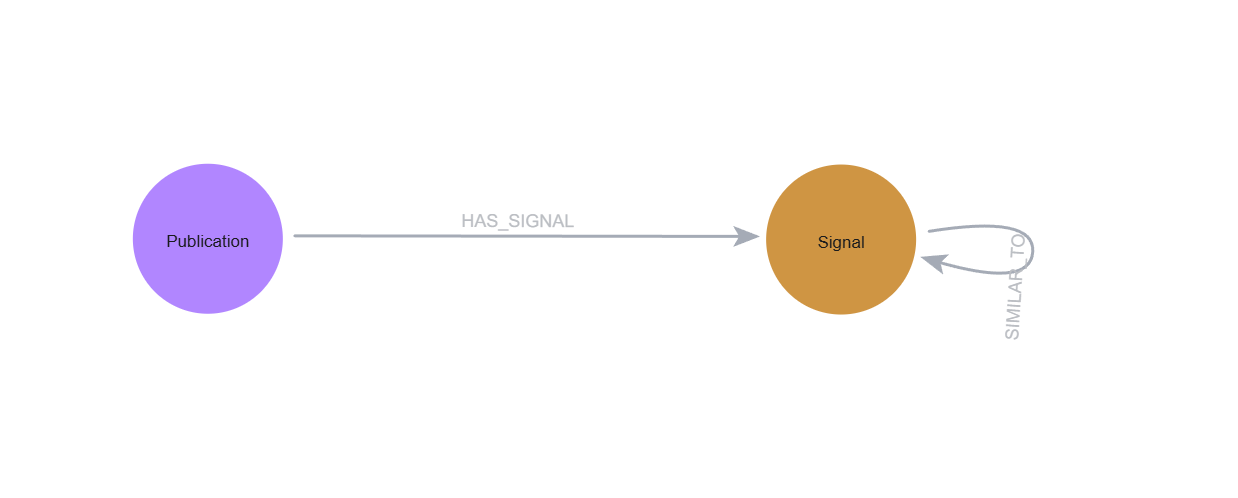
\includegraphics[width=0.85\textwidth]{figuras/graph_schema.png}
	\caption{Esquema dos nós e das relações utilizados na construção do grafo.
	\newline Fonte: Autoria própria.}
	\label{fig:esquema-grafo}
\end{figure}

\section{Caracterização das redes por período}

A construção das relações \texttt{SIMILAR\_TO} foi realizada separadamente 
para cada intervalo de análise. Essa estratégia restringiu as comparações 
semânticas aos sinais associados ao mesmo período entre reuniões 
consecutivas do FOMC, evitando a formação de relações entre sinais 
pertencentes a contextos temporais distintos.

As datas que delimitam os períodos foram obtidas da base textual 
produzida nas etapas anteriores. Foram selecionadas as publicações 
cujo título correspondia exatamente a \textit{Federal Reserve issues FOMC statement}, 
referentes aos comunicados oficiais divulgados após as reuniões do FOMC. 
As respectivas datas de publicação foram reunidas, eventuais duplicidades 
foram eliminadas e os valores foram ordenados cronologicamente.

A partir dessa sequência, cada intervalo foi definido por duas datas consecutivas 
de divulgação dos comunicados do FOMC. Para um período iniciado em $t_i$ e 
encerrado em $t_{i+1}$, foram selecionados os nós \texttt{Signal} 
que possuíam a propriedade \texttt{embedding\_signal} e 
cuja data satisfazia a condição 

\[
t_i \leq \text{data de publicação} < t_{i+1}.
\]

Consequentemente, as comunicações publicadas na data inicial foram incluídas no 
período, enquanto aquelas divulgadas na data do comunicado subsequente 
foram excluídas. Essa definição evita que o indicador referente ao 
intervalo incorpore informações publicadas simultaneamente à decisão do 
FOMC utilizada posteriormente como referência para sua avaliação, 
preservando o caráter prospectivo da análise.

A quantidade de sinais monetários disponíveis para a construção da 
rede variou entre os períodos analisados, em função do número e do 
conteúdo das comunicações publicadas entre reuniões consecutivas do FOMC. 
A Figura~\ref{fig:node_count_by_fomc_period} apresenta o número de 
nós \texttt{Signal} selecionados 
em cada intervalo. Cada nó corresponde a um sinal monetário extraído das 
comunicações publicadas entre a data inicial do período, inclusive, 
e a data do comunicado subsequente, exclusive.

\begin{figure}[H]
\centering
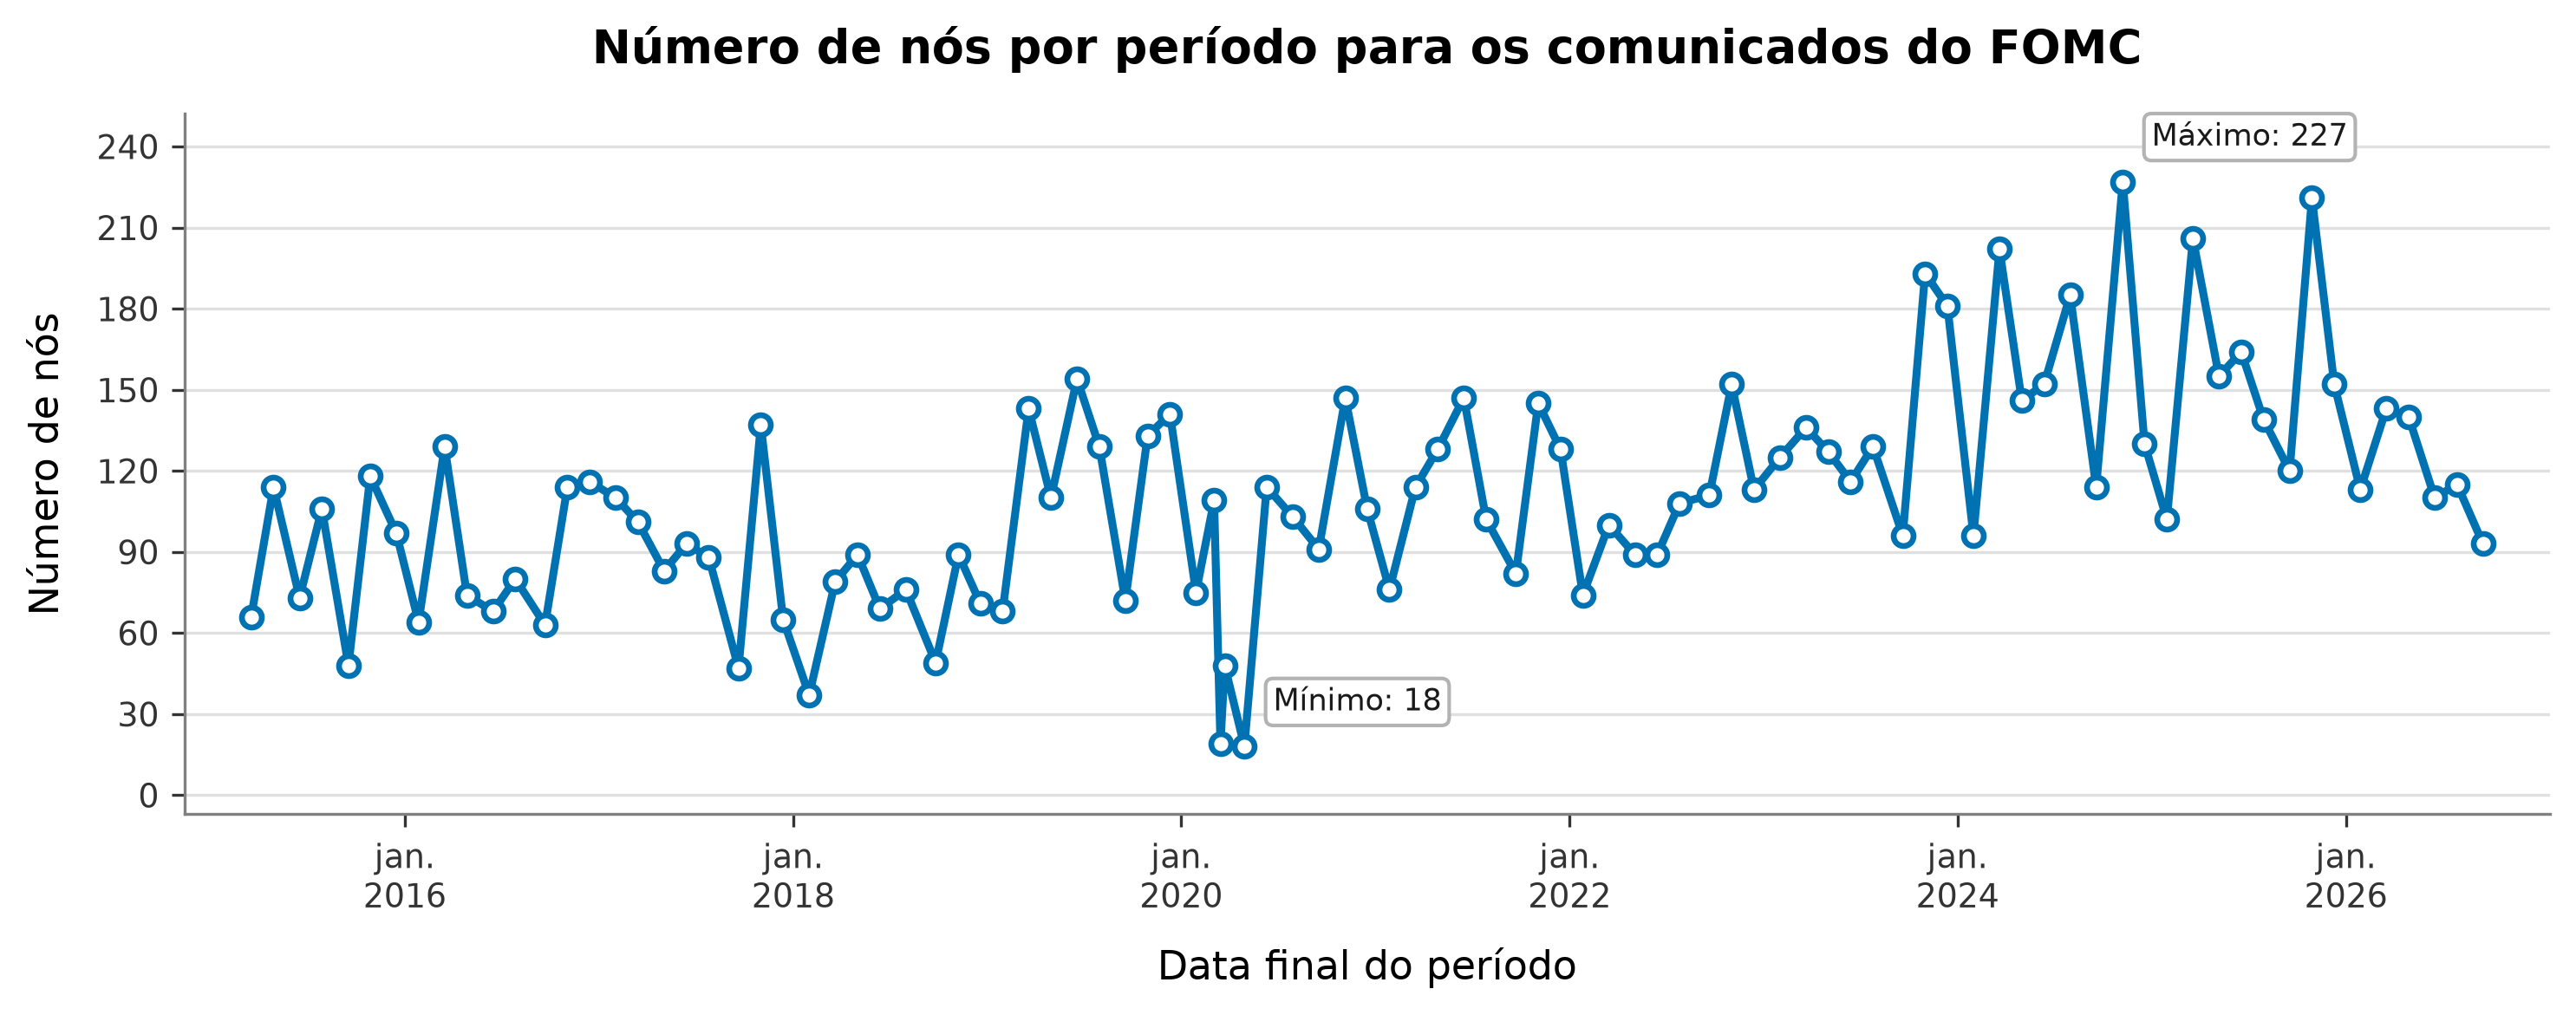
\includegraphics[width=1\textwidth]{figuras/node_count_by_fomc_period.png}
\caption{Número de sinais monetários utilizados na construção da rede em cada período entre comunicados consecutivos do FOMC.
\newline Fonte: Autoria própria.}
\label{fig:node_count_by_fomc_period}
\end{figure}

A variação no número de nós evidencia que a quantidade de 
informações disponíveis para a construção das redes não é constante 
ao longo do tempo. Sendo que o mínimo de sinais disponíveis ocorre nas reuniões
de realizadas no começo da pandemia de COVID-19.

Para cada intervalo, os sinais selecionados foram projetados temporariamente 
em memória por meio do Neo4j Graph Data Science (GDS). Na primeira projeção, 
denominada \texttt{signal-cypher}, foram incluídos apenas os nós 
\texttt{Signal} pertencentes ao período e a propriedade vetorial 
\texttt{embedding\_signal}. Essa projeção não altera a estrutura persistida 
no banco de dados e foi utilizada exclusivamente como entrada para o 
cálculo das relações de similaridade.

Sobre essa projeção foi executado o algoritmo \textit{k}-nearest neighbors (KNN). 
A comparação entre os 
sinais foi realizada utilizando a similaridade do cosseno 
aplicada aos vetores de \textit{embedding}. Para cada nó, foram 
considerados no máximo 50 vizinhos semanticamente mais 
próximos (\texttt{topK = 50}), sujeitos também a um limiar 
mínimo de similaridade.

O procedimento retornou, para cada conexão selecionada, os identificadores 
dos dois nós e o respectivo valor de similaridade. Esses identificadores 
foram convertidos novamente nos nós \texttt{Signal} armazenados no Neo4j. 
Para impedir a criação duplicada de uma mesma associação, os pares 
foram filtrados de acordo com seus identificadores internos antes 
da persistência da relação. Para cada par mantido, foi criada 
uma relação \texttt{SIMILAR\_TO}, e o valor calculado pelo KNN 
foi armazenado na propriedade \texttt{score\_similarity}.

O limiar mínimo de similaridade foi determinado de forma adaptativa 
para cada período. O procedimento foi iniciado com valor igual a 0,80. 
Após a construção das relações, uma nova projeção, 
denominada \texttt{signal-wcc}, foi formada com os nós e as conexões 
daquele intervalo, considerando as relações como não direcionadas. 
Em seguida, foi aplicado o algoritmo de componentes 
fracamente conectadas (\textit{Weakly Connected Components} - WCC) 
para determinar o número de componentes conexas existentes na rede.

Quando mais de uma componente era identificada, o limiar de 
similaridade era reduzido em 0,01 e as relações \texttt{SIMILAR\_TO} 
eram reconstruídas. O procedimento era repetido até que todos os nós 
do período pertencessem a uma única componente conexa ou até que 
fosse atingido o limite mínimo de 0,10. Dessa forma, para cada 
período foi selecionado o maior limiar, dentro da sequência 
testada, capaz de produzir uma rede conectada.

Esse procedimento procurou estabelecer um equilíbrio entre duas 
características da rede. Limiares elevados preservam apenas 
relações de maior proximidade semântica, porém podem produzir 
grupos isolados de sinais. A redução progressiva do limiar adiciona 
conexões menos semelhantes até que seja obtida uma estrutura 
conectada.

Ao final do procedimento, cada intervalo entre comunicados 
consecutivos do FOMC foi representado por uma rede semântica 
ponderada. Os nós correspondem aos sinais monetários 
identificados nas comunicações publicadas durante o período, 
enquanto as relações representam sua proximidade semântica e 
são ponderadas pela propriedade \texttt{score\_similarity}. 
Essa representação constitui a entrada para os algoritmos de 
detecção de comunidades e de centralidade empregados na construção 
dos indicadores de orientação monetária.

Os limiares de similaridade obtidos pelo procedimento 
adaptativo variaram entre os períodos analisados, refletindo 
diferenças na estrutura semântica dos sinais disponíveis em 
cada intervalo. A Figura~\ref{fig:similarity_cutoff} apresenta 
o valor do limiar necessário para que a rede correspondente 
a cada período formasse uma única componente conexa.

\begin{figure}[H]
\centering
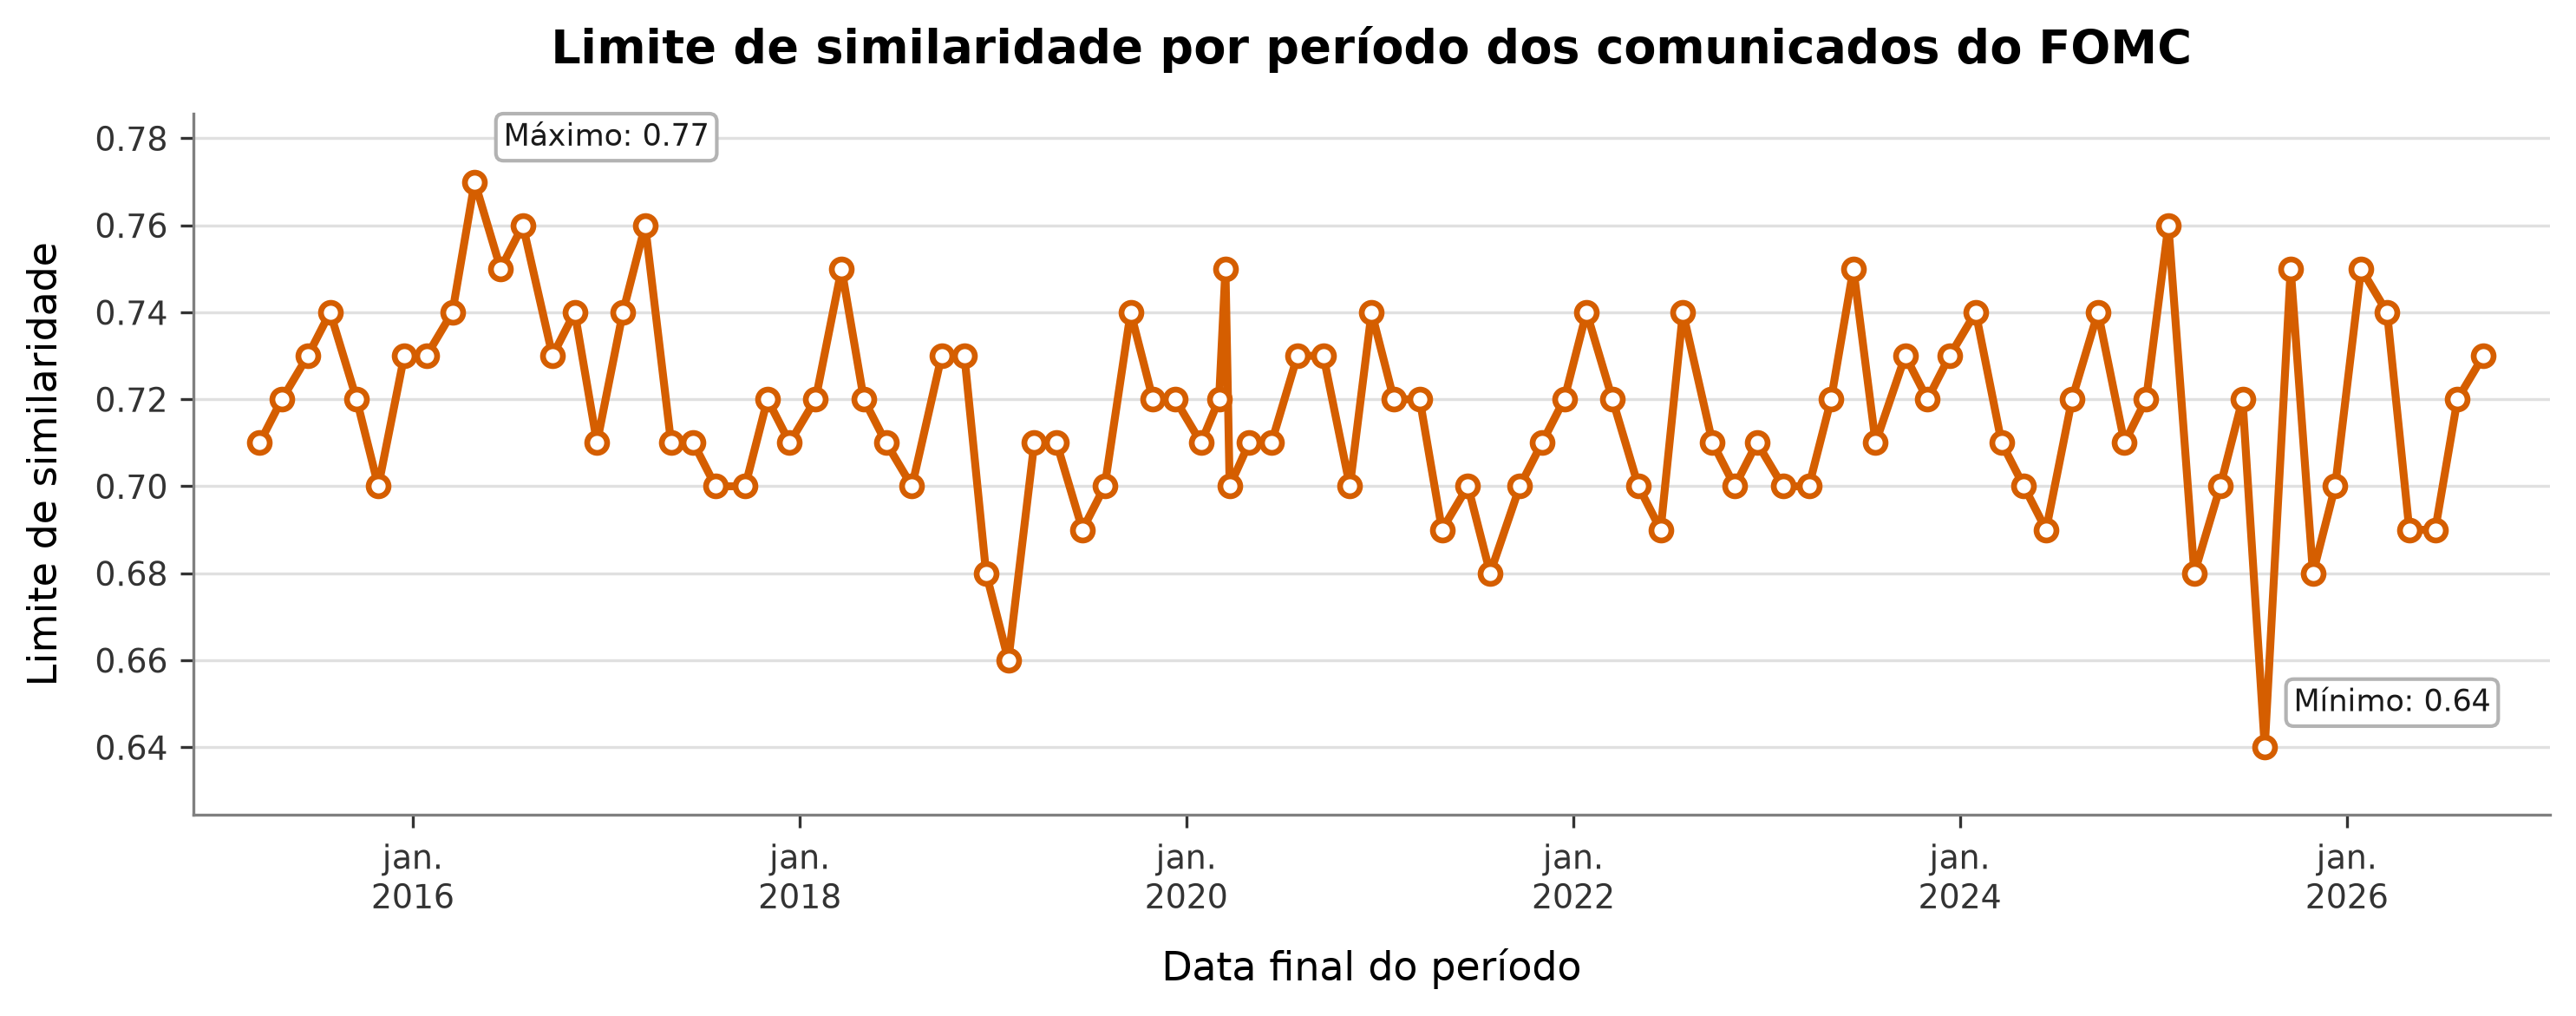
\includegraphics[width=\textwidth]{figuras/similarity_cutoff_by_fomc_period.png}
\caption{Limiar de similaridade utilizado na construção da rede em 
cada período entre comunicados consecutivos do FOMC.
\newline Fonte: Autoria própria.}
\label{fig:similarity_cutoff}
\end{figure}

Os resultados mostram que não foi necessário utilizar o 
mesmo nível mínimo de similaridade em todos os períodos 
para obter uma rede conectada. Um limiar mais elevado indica 
que os diferentes documentos apresentam pontos de vista mais 
próximos entre si, permitindo conectar os sinais com relações 
de maior proximidade semântica e preservando uma rede mais 
coesa quanto ao conteúdo abordado. Em contraste, um limiar 
mais baixo indica maior dispersão entre os pontos de vista 
expressos nos documentos: para formar uma única rede, foi 
necessário incorporar relações entre sinais progressivamente 
menos semelhantes. Assim, o limiar sintetiza o grau de 
convergência semântica necessário para conectar os sinais 
produzidos no período, sem representar diretamente a 
orientação favorável ou contrária da política monetária.

Além da abordagem com limiar de similaridade adaptativo, 
foi avaliada uma segunda configuração utilizando um limiar 
constante para todos os períodos. Para definir esse valor, 
foi calculada a mediana dos limiares de similaridade 
obtidos individualmente pelo procedimento adaptativo ao 
longo dos intervalos analisados. A mediana resultante foi 
igual a \ConstantSimilarityCutoff. Valor adotado como limiar 
fixo no segundo cenário. 
Essa escolha permite utilizar um valor representativo dos 
limiares requeridos para a formação das redes no procedimento adaptativo, 
ao mesmo tempo em que mantém constante o critério de conexão entre os sinais 
ao longo de toda a série temporal.


\section{Construção dos indicadores}

Após a construção da rede de similaridade semântica para cada período 
entre reuniões consecutivas do FOMC, foram calculadas diferentes versões 
do indicador de orientação monetária. Para isso, foram combinadas as 
pontuações atribuídas aos sinais monetários com informações 
estruturais extraídas do grafo. Foram utilizados o algoritmo de 
Leiden para detecção de comunidades e três medidas de 
centralidade: centralidade de intermediação (\textit{betweenness centrality}), 
centralidade de grau (\textit{degree centrality}) e PageRank.

Inicialmente, as três medidas de centralidade foram 
calculadas para cada nó \texttt{Signal} da rede. Os 
resultados foram associados por meio do identificador 
de cada nó, formando uma base contendo, para cada sinal, 
sua pontuação de orientação monetária (\texttt{node\_score}) 
e os respectivos valores de centralidade. 

Como referência, foi calculada a média simples das pontuações 
dos sinais pertencentes ao período. Esse indicador atribui o 
mesmo peso a todos os nós e, portanto, não incorpora informações 
sobre a posição de cada sinal na estrutura da rede. 
Sua expressão pode ser representada por

\[
I_{\text{média}} =
\frac{1}{N}\sum_{i=1}^{N}s_i,
\]

em que $s_i$ representa a pontuação de orientação monetária 
do sinal $i$ e $N$ corresponde ao número de sinais 
considerados no período.

Em seguida, foram construídos três indicadores utilizando as 
medidas de centralidade como fatores de ponderação. De forma geral, 
para uma medida de centralidade $c_i$, o indicador foi calculado por

\[
I_c =
\frac{\sum_{i=1}^{N}s_i c_i}
{\sum_{i=1}^{N}c_i}.
\]

A primeira ponderação utilizou a centralidade de intermediação. 
Essa medida destaca sinais que ocupam posições de intermediação 
na rede, isto é, nós que participam com maior frequência dos 
caminhos que conectam diferentes regiões do grafo. 
Dessa forma, sinais com maior centralidade de intermediação 
receberam maior peso na composição do indicador 
\texttt{betweenness\_weighted\_sentiment}.

A segunda versão utilizou a centralidade de grau ponderado. 
Nesse caso, o peso atribuído a cada sinal decorre da intensidade 
de suas conexões com os demais nós da rede, 
produzindo o indicador \texttt{degree\_weighted\_sentiment}. 
Essa abordagem atribui maior influência aos sinais que apresentam 
maior relevância local na estrutura de similaridade semântica.

A terceira ponderação foi realizada utilizando o PageRank. 
Essa medida considera a relevância estrutural do nó 
levando em conta não apenas suas próprias conexões, 
mas também a relevância dos nós aos quais ele está conectado. 
Os valores calculados pelo algoritmo foram utilizados como pesos 
das pontuações monetárias, resultando no indicador 
\texttt{pagerank\_weighted\_sentiment}.


As Figuras~\ref{fig:variable_cutoff} e
\ref{fig:fixed_cutoff} apresentam a evolução temporal para Leiden e dos 
três indicadores ponderados por centralidade. A primeira 
corresponde às redes construídas com limiar de similaridade 
variável entre os períodos, enquanto a segunda utiliza o l
imiar fixo de \ConstantSimilarityCutoff.

\begin{figure}[H]
\centering
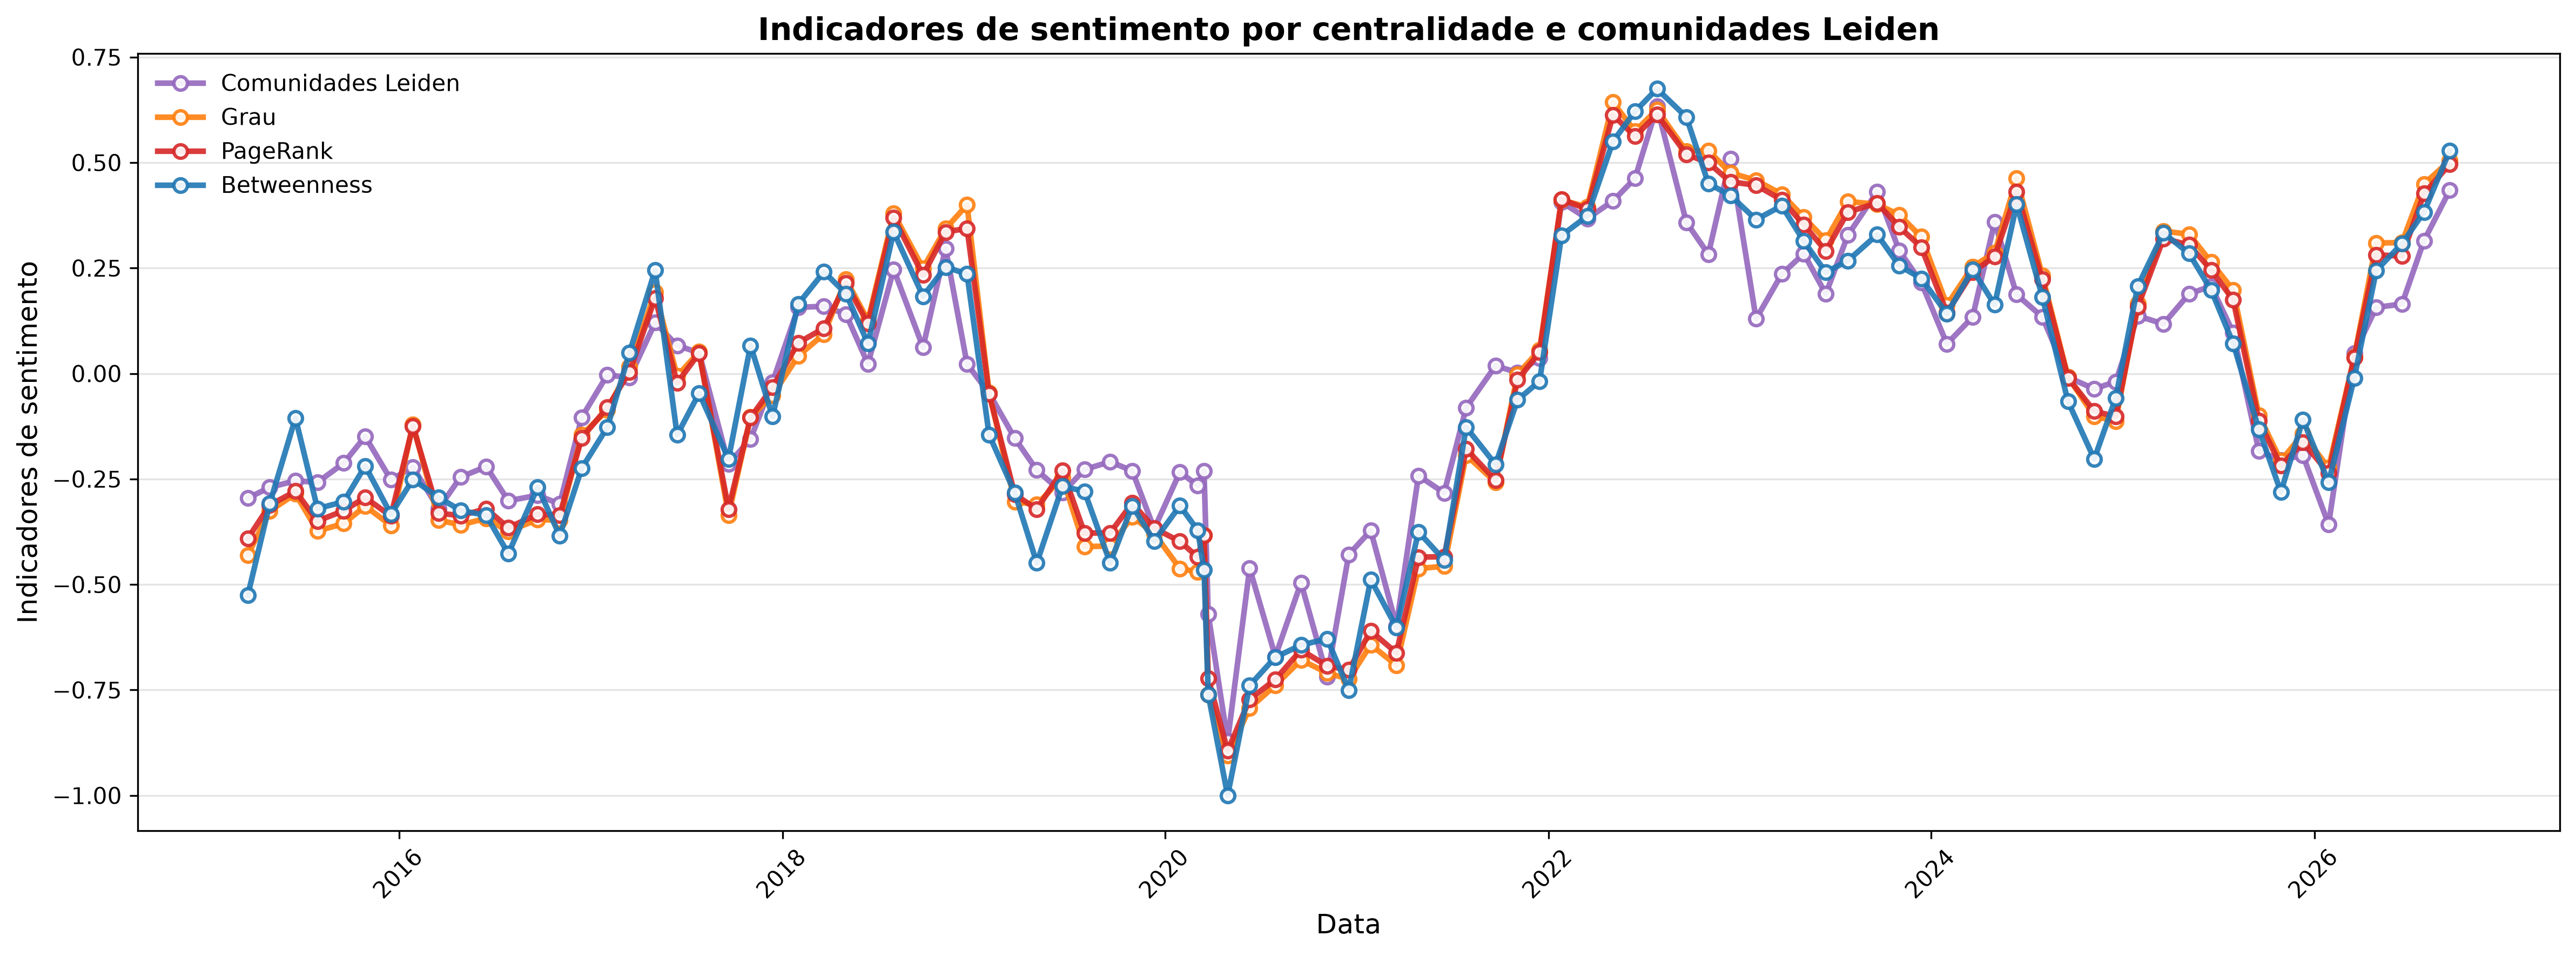
\includegraphics[width=1\textwidth]{figuras/sentiment_indicators_centrality_by_fomc_period.png}
\caption{Indicadores de orientação monetária obtidos usando Leiden 
e medidas de centralidade de intermediação, grau e 
PageRank para as redes construídas com limiar de 
similaridade variável.
\newline Fonte: Autoria própria.}
\label{fig:variable_cutoff}
\end{figure}

\begin{figure}[H]
\centering
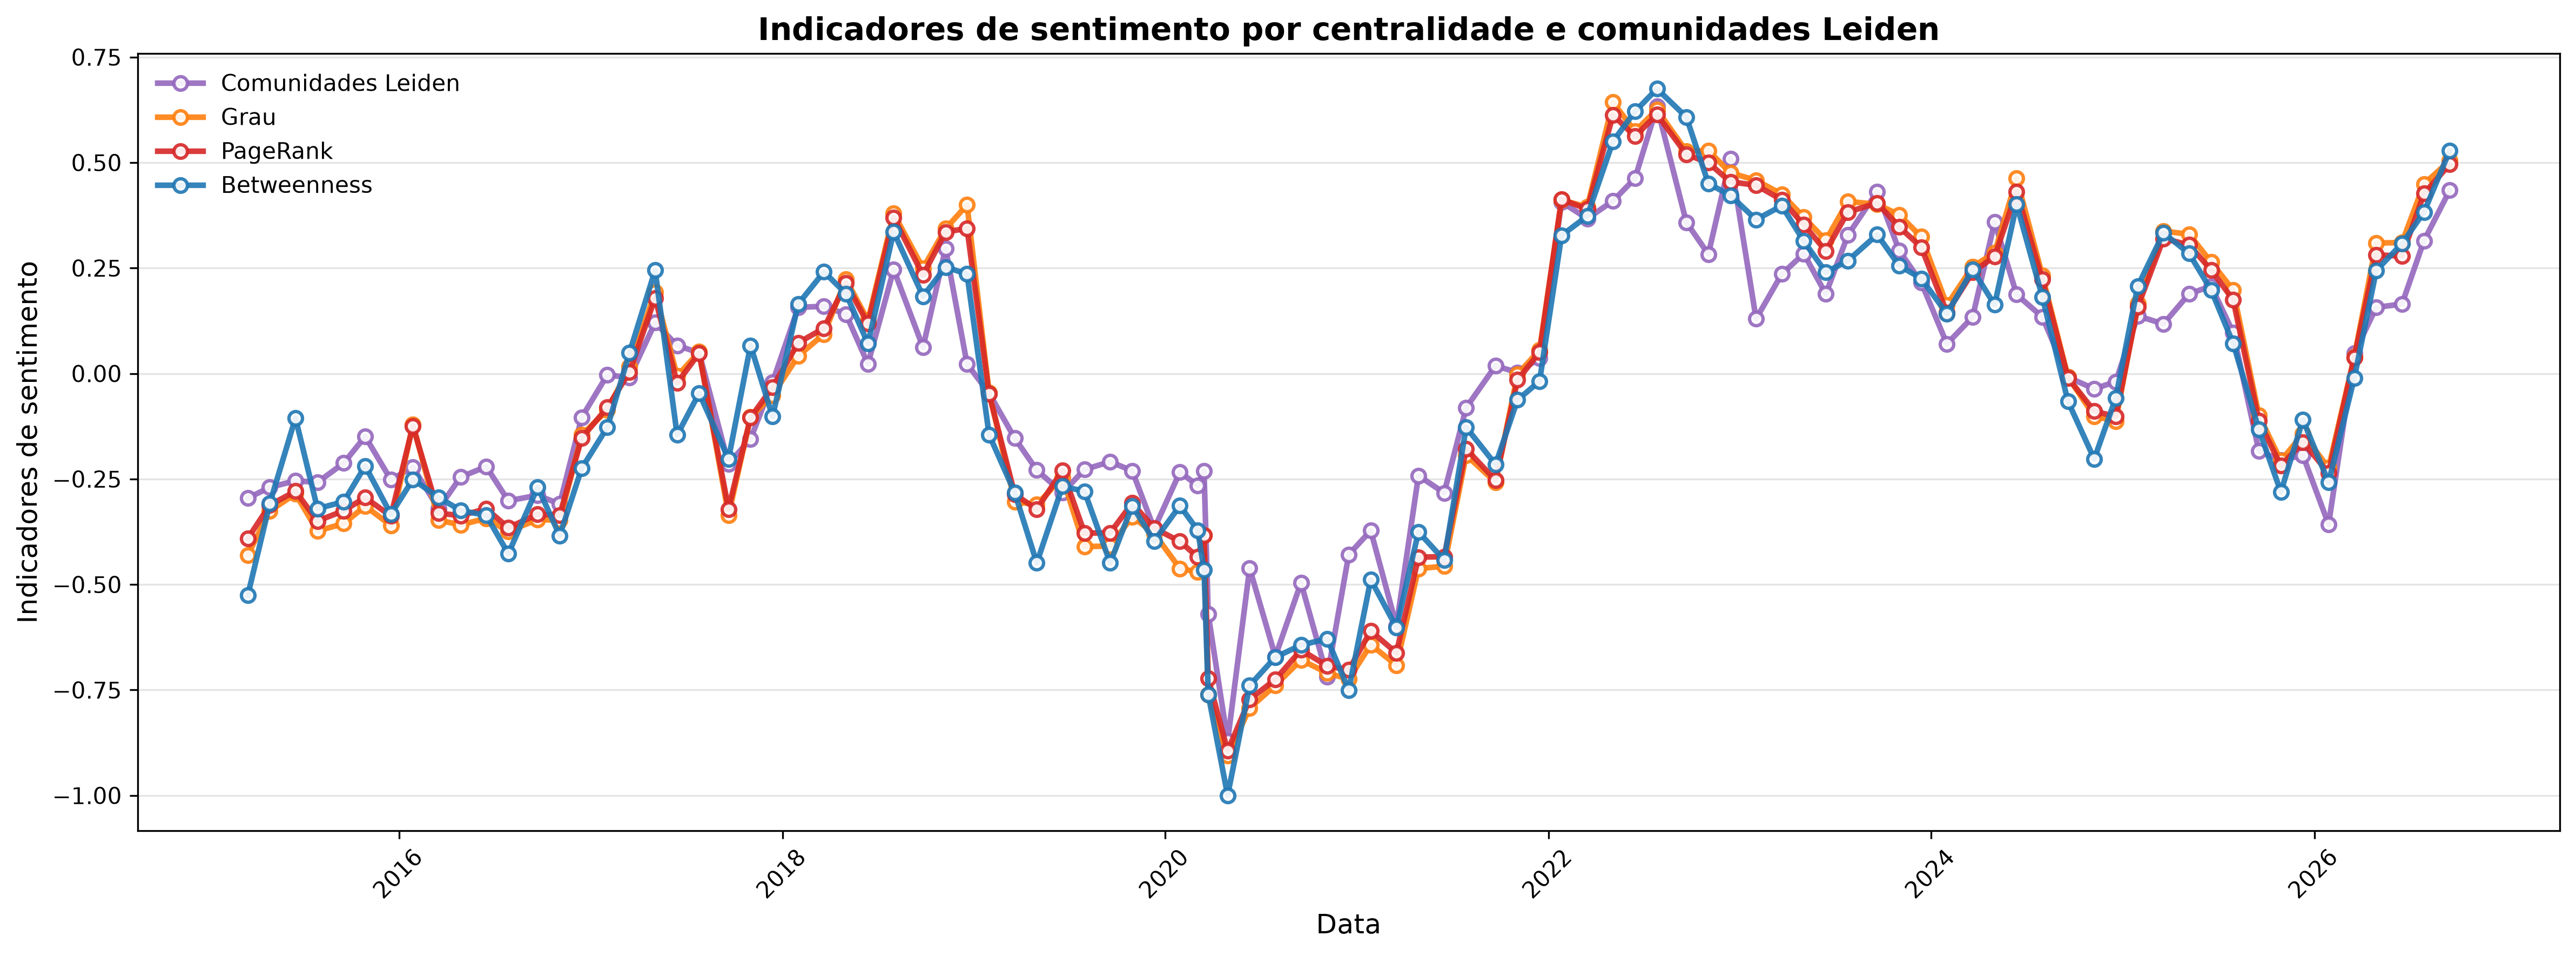
\includegraphics[width=1\textwidth]{figuras/sentiment_indicators_centrality_by_fomc_period_fixed.png}
\caption{Indicadores de orientação monetária obtidos pela média 
simples e pelas medidas de centralidade de intermediação, grau e 
PageRank para as redes construídas com limiar fixo de 
similaridade igual a \ConstantSimilarityCutoff.
\newline Fonte: Autoria própria.}
\label{fig:fixed_cutoff}
\end{figure}

Além dos indicadores calculados diretamente sobre todos os nós da rede, 
o algoritmo de Leiden foi utilizado para incorporar a estrutura 
de comunidades à agregação dos sinais. Para cada período, o 
algoritmo associou cada nó a uma comunidade, permitindo 
separar a rede em grupos de sinais semanticamente 
relacionados.


A primeira medida baseada em Leiden foi construída 
calculando-se, inicialmente, a média simples da pontuação dos 
sinais pertencentes a cada comunidade. Posteriormente, 
as médias das comunidades foram agregadas com pesos iguais, conforme

\[
I_{\text{Leiden}} =
\frac{1}{K}
\sum_{k=1}^{K}
\left(
\frac{1}{N_k}
\sum_{i \in C_k}s_i
\right),
\]

em que $K$ representa o número de comunidades identificadas, 
$C_k$ corresponde à comunidade $k$ e $N_k$ representa seu número 
de sinais. O resultado corresponde ao indicador 
\texttt{leiden\_equal\_weight\_sentiment}. Esse procedimento 
faz com que cada comunidade contribua igualmente para o resultado 
final, independentemente de sua quantidade de nós.


Também foram construídas três versões que combinam a detecção de 
comunidades com as medidas de centralidade. Nesse procedimento, 
a ponderação pelas centralidades foi realizada inicialmente 
dentro de cada comunidade. Para uma medida de centralidade $c$, 
a orientação monetária da comunidade $k$ foi calculada como

\[
I_{k,c} =
\frac{
\sum_{i \in C_k}s_i c_i
}{
\sum_{i \in C_k}c_i
}.
\]

Após o cálculo individual para cada comunidade, os valores obtidos 
foram agregados por meio de uma média simples entre as comunidades:

\[
I_{\text{Leiden},c} =
\frac{1}{K}
\sum_{k=1}^{K} I_{k,c}.
\]

Dessa combinação resultaram três indicadores: um baseado na centralidade
de intermediação, outro na centralidade de grau e o terceiro no PageRank.
Em cada caso, a importância estrutural dos sinais é calculada dentro de
cada comunidade. Posteriormente, os valores das comunidades são agregados
por meio de uma média simples, de modo que todas recebam o mesmo peso no
indicador final. Essa abordagem diferencia esses indicadores daqueles
calculados diretamente sobre toda a rede.


As Figuras~\ref{fig:sentiment_indicators_centrality_community_by_fomc_period} e
\ref{fig:sentiment_indicators_centrality_community_by_fomc_period_fixed} 
apresentam os indicadores resultantes da incorporação das 
comunidades de Leiden ao processo de agregação. Novamente, são 
apresentados separadamente os resultados produzidos pelas redes 
construídas com limiar variável e com limiar fixo de similaridade.

\begin{figure}[H]
\centering
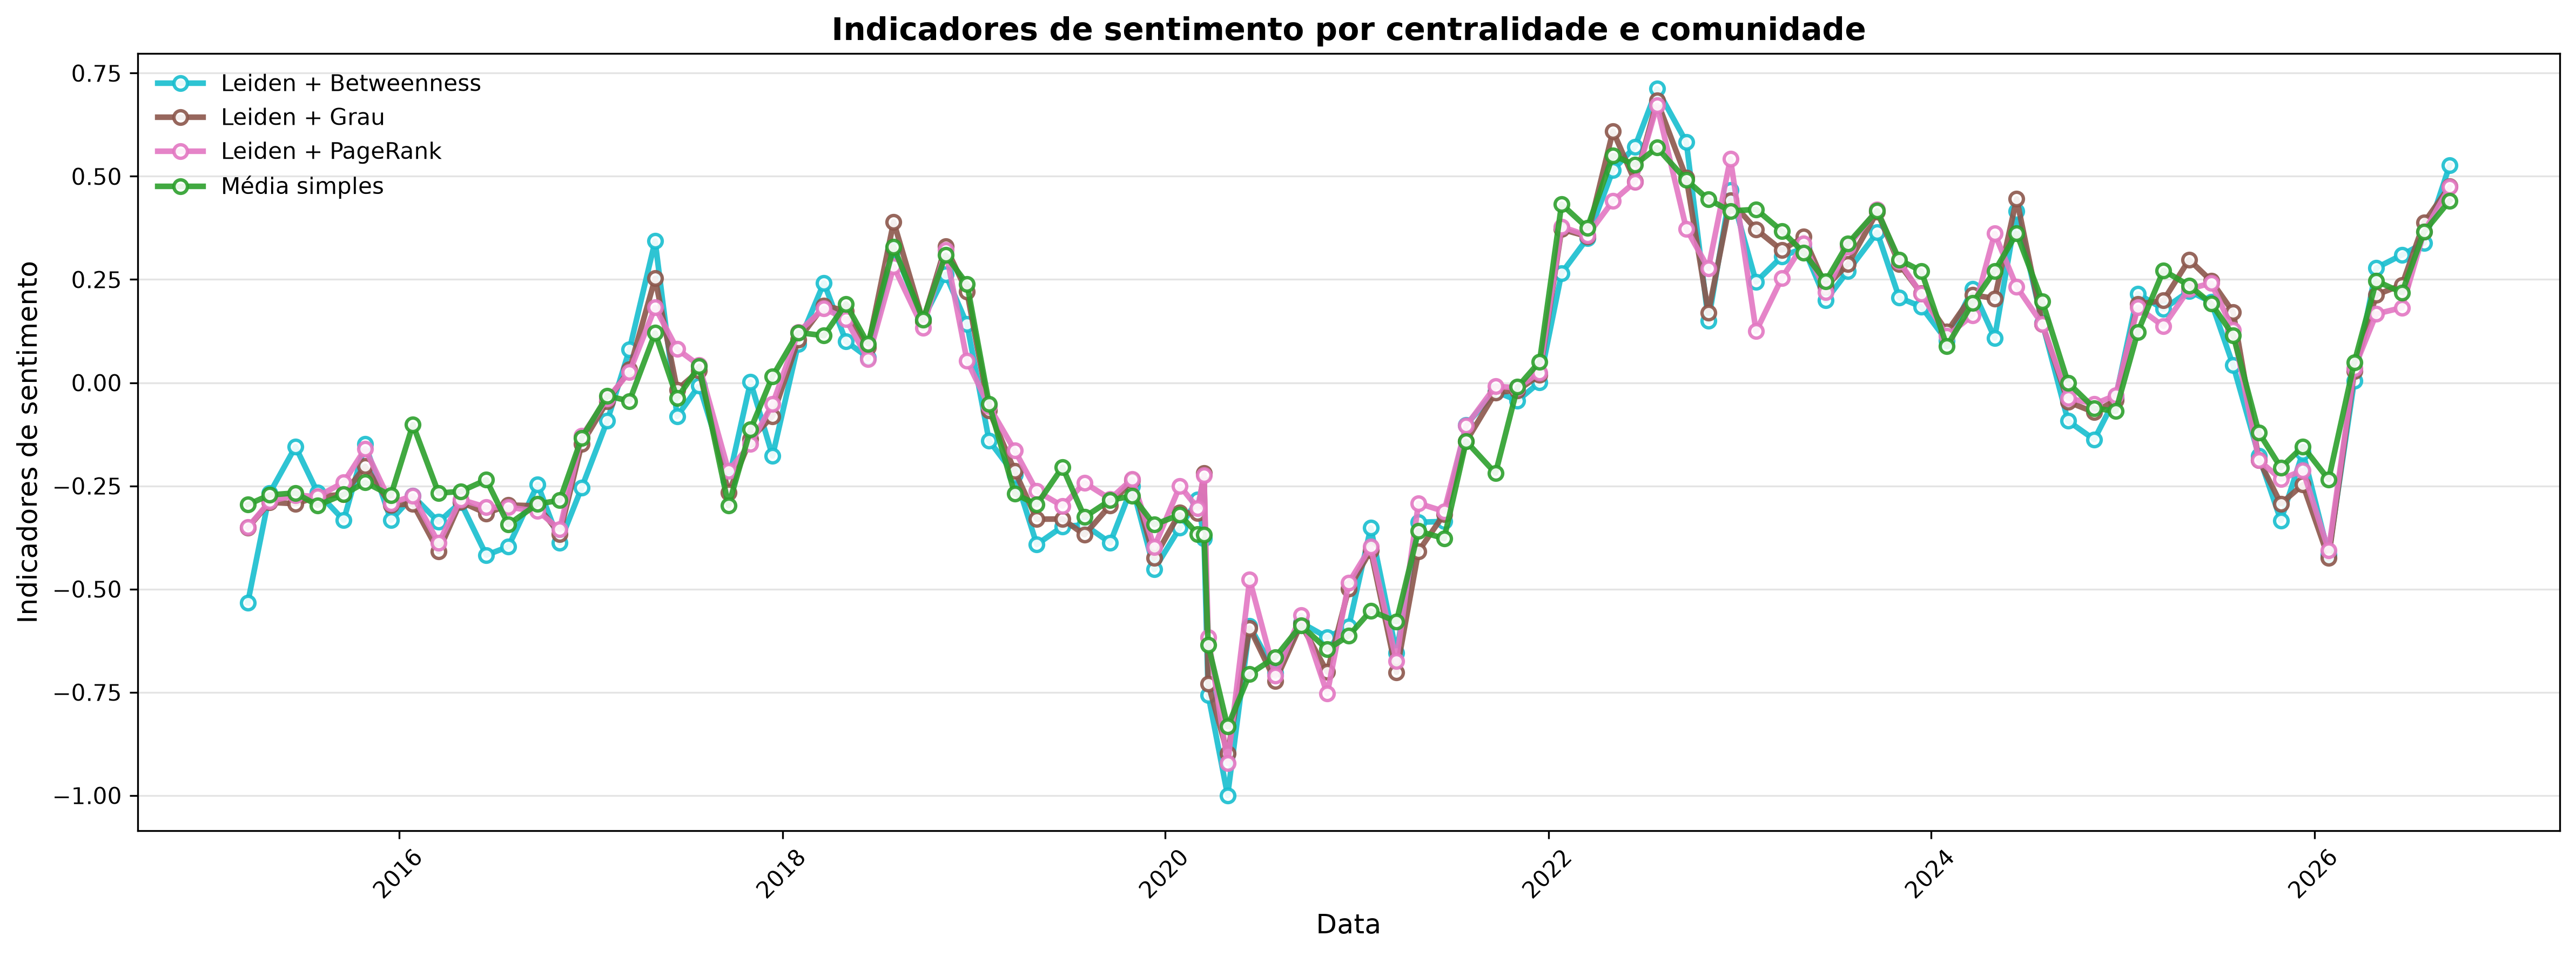
\includegraphics[width=1\textwidth]{figuras/sentiment_indicators_centrality_community_by_fomc_period.png}
\caption{Indicadores construídos a partir das comunidades identificadas 
pelo algoritmo de Leiden combinadas com as medidas de centralidade para as
redes com limiar de similaridade variável.
\newline Fonte: Autoria própria.}
\label{fig:sentiment_indicators_centrality_community_by_fomc_period}
\end{figure}

\begin{figure}[H]
\centering
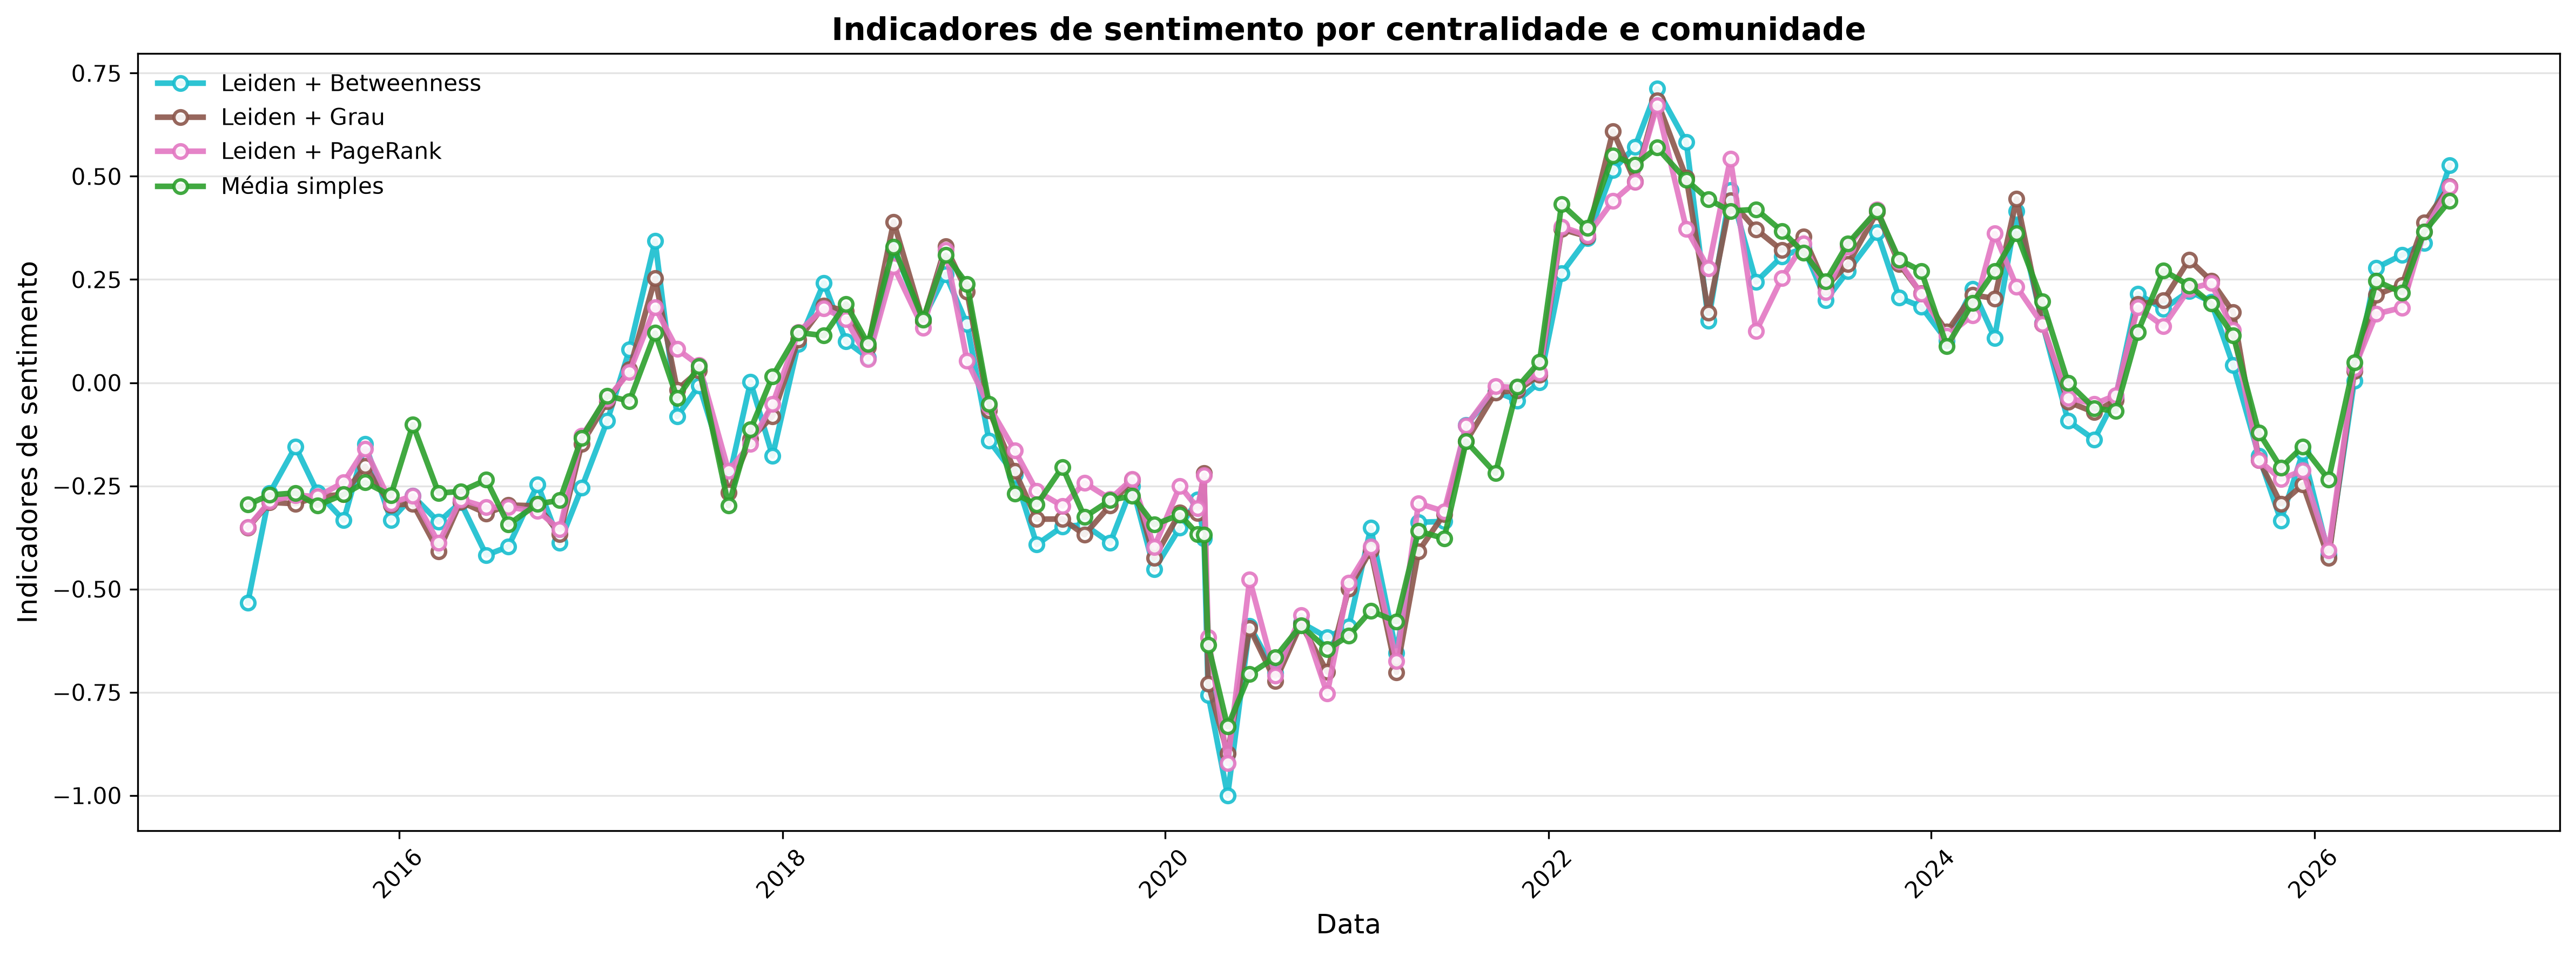
\includegraphics[width=1\textwidth]{figuras/sentiment_indicators_centrality_community_by_fomc_period_fixed.png}
\caption{Indicadores construídos a partir das comunidades identificadas 
pelo algoritmo de Leiden combinadas com as medidas de centralidade para as 
redes com limiar fixo de similaridade igual a \ConstantSimilarityCutoff.
\newline Fonte: Autoria própria.}
\label{fig:sentiment_indicators_centrality_community_by_fomc_period_fixed}
\end{figure}

Ao todo, foram obtidas oito formas de agregação da 
orientação monetária em cada período: a média simples; 
três indicadores ponderados diretamente pelas centralidades 
de intermediação, grau e PageRank; 
o indicador de comunidades de Leiden com pesos iguais; 
e três indicadores que combinam Leiden com as respectivas 
medidas de centralidade. Essa estrutura permite comparar 
uma agregação que utiliza exclusivamente as classificações 
individuais com diferentes formas de incorporação da 
organização estrutural e semântica da rede. Além disso, 
os mesmos algoritmos e procedimentos de cálculo foram 
utilizados nas duas estratégias de construção das redes 
consideradas neste trabalho. 


\section{Obtenção da \textit{Federal Funds Rate}}

Para avaliar a relação entre os indicadores de orientação 
monetária e as decisões 
posteriores do Federal Open Market Committee (FOMC), 
foram obtidas informações 
referentes à faixa-alvo da Federal Funds Rate. 
Os dados foram consultados por meio 
da API do Federal Reserve Economic Data (FRED), 
utilizando duas séries temporais: 
\texttt{DFEDTARL}, correspondente ao limite 
inferior da faixa-alvo, e 
\texttt{DFEDTARU}, correspondente ao limite superior.

Como a análise deste trabalho é organizada de acordo 
com os períodos delimitados 
pelos comunicados das reuniões do FOMC, foram mantidas 
apenas as observações da 
taxa de juros cujas datas coincidiam com as datas de 
publicação dos comunicados 
\textit{Federal Reserve issues FOMC statement}. 
Dessa forma, a série diária 
original foi reduzida às observações correspondentes 
às decisões de política 
monetária utilizadas como referência na análise.

Para representar a mudança na política de juros entre 
reuniões consecutivas, foi 
utilizado o limite superior da faixa-alvo. 
Para uma reunião ocorrida na data $t$, 
a variação foi calculada pela diferença entre o 
limite superior observado nessa 
data e o limite superior correspondente à reunião anterior:

\[
\Delta r_t = r_t^{U} - r_{t-1}^{U},
\]

em que $r_t^{U}$ representa o limite superior da 
faixa-alvo da Federal Funds Rate 
na data $t$ e $r_{t-1}^{U}$ representa o limite 
superior observado na reunião 
anterior.


Assim, valores positivos de $\Delta r_t$ representam 
elevação do limite superior 
da faixa-alvo entre duas reuniões consecutivas, 
valores negativos representam 
redução e valores iguais a zero indicam manutenção. 
Para a primeira observação da 
série, para a qual não existe uma reunião anterior 
disponível para o cálculo da 
diferença, o valor foi preenchido com zero.

A evolução da variação do limite superior da faixa-alvo 
ao longo das reuniões
do FOMC é apresentada na Figura~\ref{fig:upper_rate_change}. 
Os valores
positivos indicam elevações da taxa, enquanto 
os valores negativos representam
reduções entre reuniões consecutivas.

\begin{figure}[H]
\centering
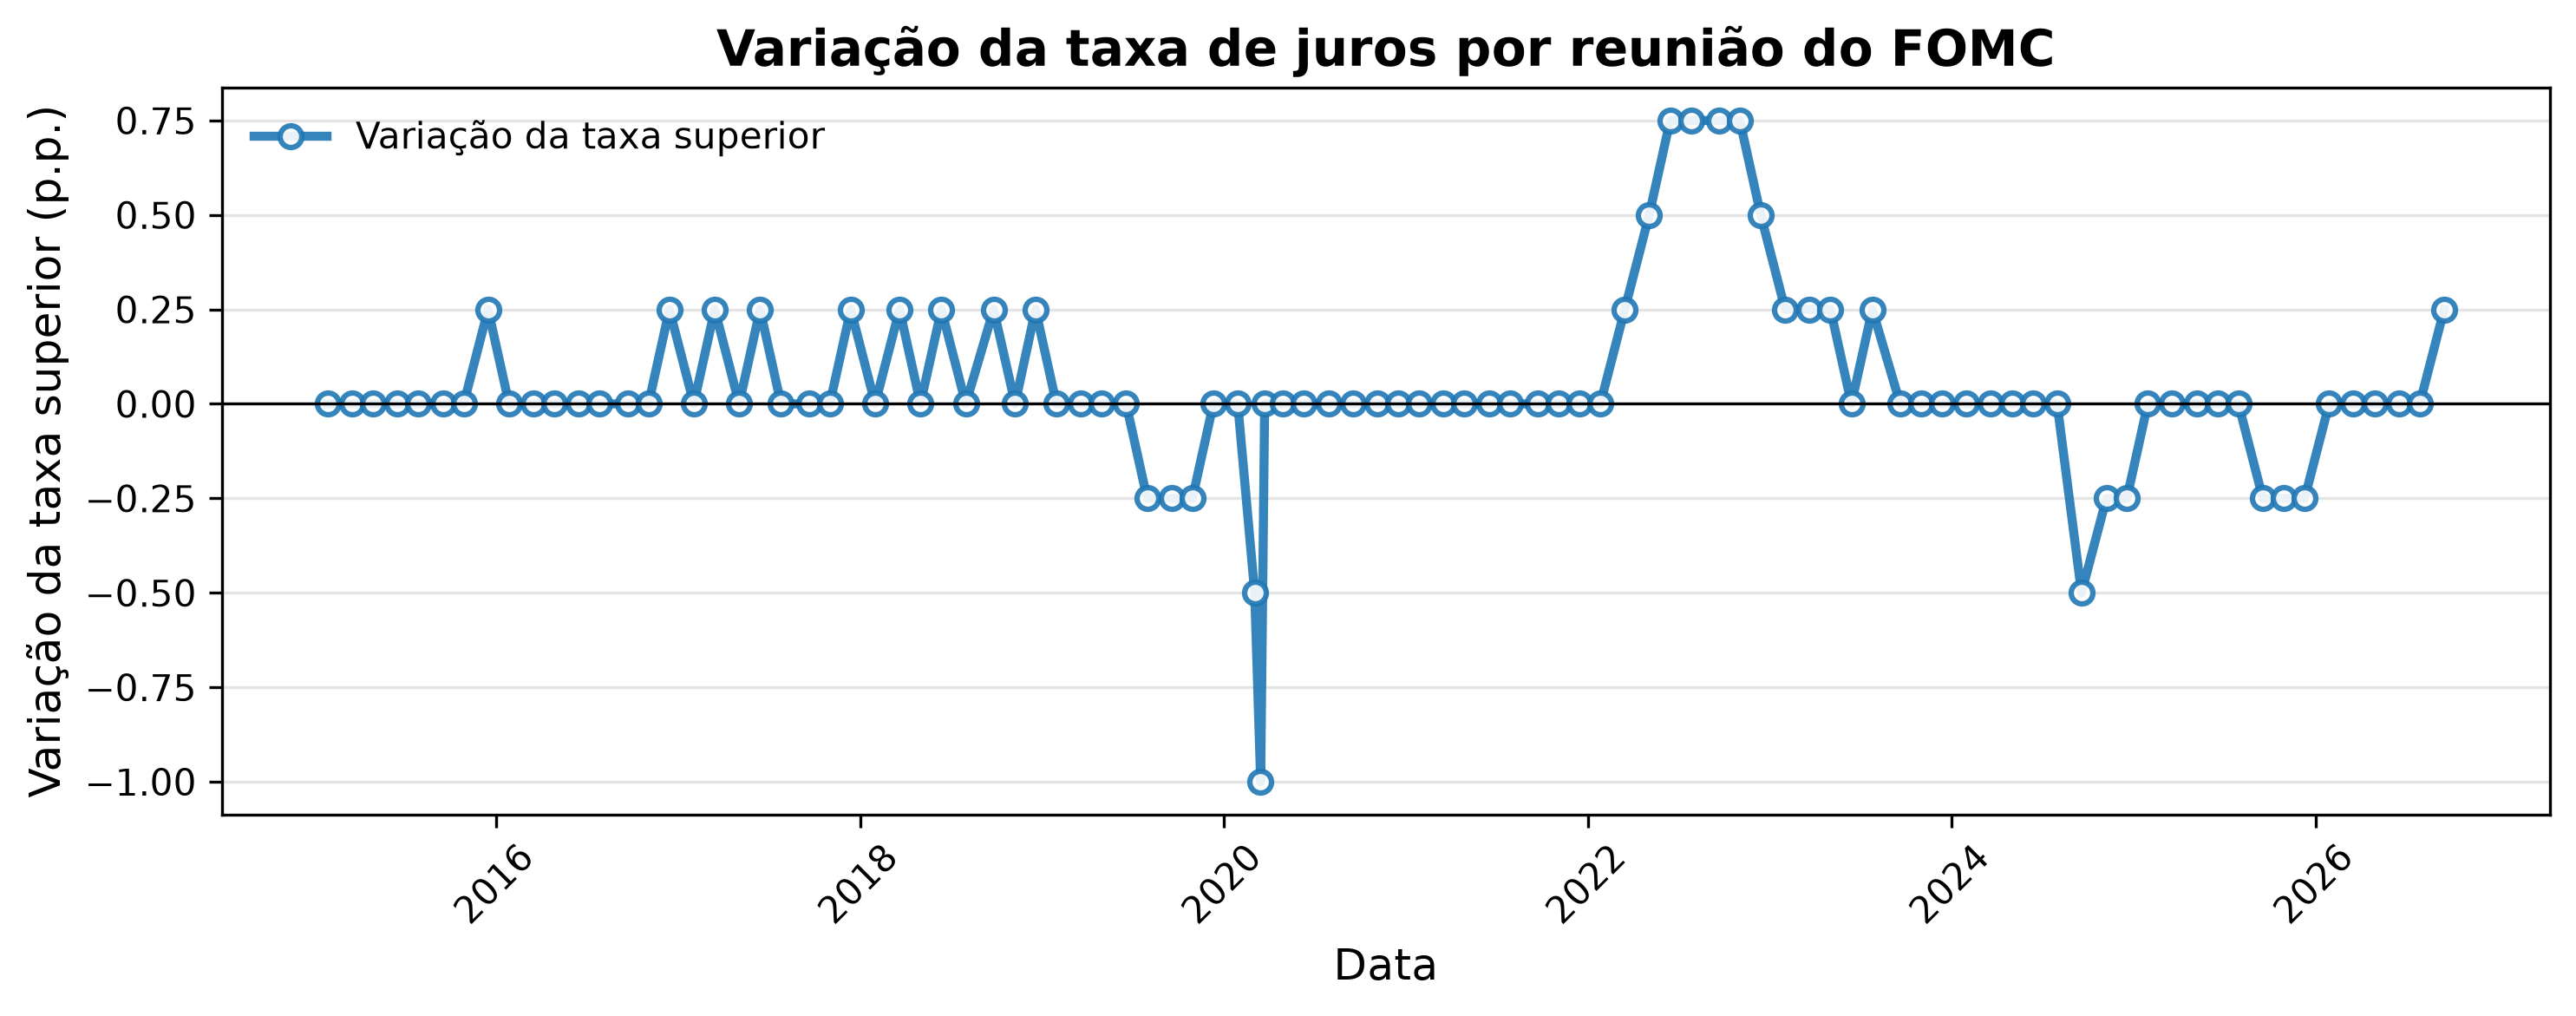
\includegraphics[width=1\textwidth]{figuras/upper_rate_change_by_fomc_period.png}
\caption{Variação do limite superior da faixa-alvo 
da Federal Funds Rate entre reuniões 
consecutivas do FOMC.
\newline Fonte: Autoria própria.}
\label{fig:upper_rate_change}
\end{figure}


\section{Correlação entre os Indicadores e a Variação da \textit{Federal Funds Rate}}

Para avaliar a associação entre a orientação monetária identificada nas 
comunicações do Federal Reserve e a variação do limite superior da faixa-alvo da 
\textit{Federal Funds Rate}, representada por $\Delta r_t$, foram calculados os 
coeficientes de correlação de Pearson e de Spearman. A correlação de Pearson 
mede a associação linear entre as variáveis, enquanto a correlação de Spearman 
avalia a relação monotônica a partir das posições relativas das observações. 
Foram considerados os indicadores construídos com limiar de similaridade variável 
e com limiar fixo de $0,72$. Os resultados são apresentados na 
Tabela~\ref{tab:correlacoes-upper-rate-change}.

\begin{table}[htbp]
\centering
\caption{Correlações entre os indicadores de orientação monetária e a variação do 
limite superior da \textit{Federal Funds Rate}.}
\label{tab:correlacoes-upper-rate-change}

\begin{tabular}{lcccc}
\hline
& \multicolumn{2}{c}{\textbf{Limiar variável}} & \multicolumn{2}{c}{\textbf{Limiar fixo}} \\
\textbf{ } & \textbf{Pearson} & \textbf{Spearman} & \textbf{Pearson} & \textbf{Spearman} \\
\hline
Betweenness & 0,460 & 0,460 & 0,503 & 0,483 \\
Grau & 0,475 & 0,495 & 0,477 & 0,501 \\
PageRank & 0,477 & 0,495 & 0,480 & 0,497 \\
Comunidades Leiden & 0,495 & 0,468 & 0,451 & 0,436 \\
Leiden + Betweenness & 0,458 & 0,438 & 0,476 & 0,460 \\
Leiden + Grau & 0,486 & 0,477 & 0,448 & 0,451 \\
Leiden + PageRank & 0,486 & 0,473 & 0,449 & 0,440 \\
Média simples & 0,485 & 0,497 & 0,485 & 0,497 \\
\hline
\end{tabular}

\medskip
\makebox[\textwidth][l]{Fonte: Autoria própria.}
\end{table}

Todos os coeficientes apresentados são positivos. Esse resultado indica que 
valores mais elevados dos indicadores, associados a uma orientação relativamente 
mais \textit{hawkish} nas comunicações, estiveram associados a variações maiores 
do limite superior da taxa. De forma análoga, valores mais baixos dos indicadores, 
associados a uma orientação relativamente mais \textit{dovish}, estiveram 
associados a variações menores ou negativas da taxa.

Com limiar variável, as correlações de Pearson variaram entre 0,458 e 0,495, e as 
de Spearman entre 0,438 e 0,497. O maior valor de Pearson foi observado para o 
indicador baseado nas comunidades identificadas pelo algoritmo de Leiden (0,495), 
enquanto o maior valor de Spearman foi obtido pela média simples (0,497). Os 
indicadores Grau e PageRank também apresentaram valores elevados de Spearman, 
ambos iguais a 0,495.

Com limiar fixo de $0,72$, os coeficientes de Pearson variaram entre 0,448 e 0,503, 
e os de Spearman entre 0,436 e 0,501. O maior valor de Pearson foi obtido pelo 
indicador ponderado pela centralidade de intermediação (\textit{Betweenness}), com 
0,503. Para Spearman, o maior coeficiente foi observado no indicador ponderado por 
Grau, com 0,501, seguido pelos indicadores de média simples e PageRank, ambos com 
0,497.

A comparação entre as duas medidas mostra que os resultados permanecem positivos, 
mas a magnitude varia conforme o indicador e o critério de construção da rede. A 
proximidade entre os coeficientes de Pearson e Spearman para vários indicadores 
sugere que parte da associação observada também é monotônica, embora não permita 
concluir que a relação seja estritamente linear. A escolha entre limiar variável e 
fixo também não produziu uma alteração uniforme: o limiar fixo favoreceu, por 
exemplo, os indicadores Betweenness e Leiden + Betweenness, enquanto o limiar 
variável apresentou valores maiores para os indicadores baseados nas comunidades 
de Leiden.

Por fim, esses resultados devem ser interpretados como evidência de associação 
entre as variáveis. Nenhum dos coeficientes permite estabelecer causalidade e, 
isoladamente, as correlações não demonstram capacidade preditiva dos indicadores.




\section{Avaliação da utilidade e da capacidade preditiva dos indicadores}

A correlação apresentada na seção anterior indica a existência de associação
positiva entre os indicadores de orientação monetária e a variação subsequente da
faixa-alvo da \textit{Federal Funds Rate}. Entretanto, a existência de correlação,
isoladamente, não permite determinar se os indicadores apresentam utilidade para
antecipar as decisões do FOMC ou se a incorporação da estrutura do grafo acrescenta
informação em relação à média simples das classificações. Para investigar essas
questões, foram realizadas três análises complementares: regressões com erros-padrão
robustos, avaliação do valor incremental dos indicadores de grafo e validação temporal
fora da amostra.





\subsection{Relação dos indicadores com a decisão subsequente}

Inicialmente, foram estimados modelos de regressão linear relacionando cada indicador
calculado no período entre duas reuniões consecutivas do FOMC com a variação da taxa
observada na reunião seguinte. Para um indicador $I_t$, o modelo pode ser representado
por

\[
\Delta r_{t+1} = \alpha + \beta I_t + \varepsilon_t,
\]

em que $\Delta r_{t+1}$ corresponde à variação do limite superior da faixa-alvo
observada ao final do período. As regressões foram estimadas utilizando erros-padrão
robustos à heterocedasticidade e à autocorrelação pelo procedimento HAC de
Newey-West, considerando uma defasagem.

A mesma análise foi realizada para as redes construídas com limiar de similaridade
variável e com limiar fixo de 0,72. Foram utilizadas 95 observações em cada
configuração. Os principais resultados são apresentados na
Tabela~\ref{tab:regressao-decisao-seguinte}.

\begin{table}[H]
\centering
\caption{Regressões entre os indicadores de orientação monetária e a variação da
taxa na reunião subsequente do FOMC.}
\label{tab:regressao-decisao-seguinte}
\begin{tabular}{lcccc}
\hline
& \multicolumn{2}{c}{\textbf{Limiar variável}} &
\multicolumn{2}{c}{\textbf{Limiar fixo}} \\
\cline{2-5}
\textbf{Indicador} &
$\boldsymbol{\beta}$ & $\boldsymbol{R^2}$ &
$\boldsymbol{\beta}$ & $\boldsymbol{R^2}$ \\
\hline
Betweenness            & 0,313 & 0,211 & 0,337 & 0,253 \\
Grau                   & 0,300 & 0,225 & 0,299 & 0,228 \\
PageRank               & 0,313 & 0,228 & 0,314 & 0,231 \\
Comunidades Leiden     & 0,385 & 0,245 & 0,372 & 0,204 \\
Leiden + Betweenness   & 0,325 & 0,210 & 0,337 & 0,227 \\
Leiden + Grau          & 0,339 & 0,236 & 0,318 & 0,200 \\
Leiden + PageRank      & 0,348 & 0,236 & 0,342 & 0,202 \\
Média simples          & 0,356 & 0,236 & 0,356 & 0,236 \\
\hline
\end{tabular}

\medskip
\makebox[\textwidth][l]{Fonte: Autoria própria.}
\end{table}

Todos os coeficientes estimados foram positivos e estatisticamente diferentes de
zero, com valores de $p$ corrigidos pelo procedimento HAC inferiores ou iguais a
0,001. Esse resultado indica que valores mais elevados dos indicadores, associados
a uma orientação mais \textit{hawkish}, estão relacionados a variações posteriores
mais elevadas da taxa de juros.

No cenário com limiar variável, o indicador baseado nas comunidades de Leiden
apresentou o maior coeficiente estimado ($\beta = 0,385$) e também o maior
coeficiente de determinação entre os modelos individuais ($R^2 = 0,245$). Na
configuração com limiar fixo, o maior $R^2$ foi observado para o indicador baseado
na centralidade de intermediação ($R^2 = 0,253$).

Como teste adicional, os mesmos indicadores foram relacionados à decisão observada
na reunião que marca o início de cada período. Em todas as versões avaliadas, a
associação com essa decisão anterior foi superior àquela observada para a reunião
seguinte, tanto em magnitude do coeficiente quanto em poder explicativo. Portanto,
embora os indicadores apresentem associação estatisticamente significativa com a
decisão subsequente, os resultados não indicam que sua relação seja mais forte com
a decisão futura do que com a decisão já observada no início do período.

Esse comportamento sugere cautela ao interpretar os indicadores como instrumentos
de antecipação. Parte da informação capturada ao longo de cada intervalo pode estar
associada à continuidade da orientação monetária vigente e às comunicações
produzidas após a reunião que inicia o período.

\subsection{Valor incremental da estrutura do grafo}

Uma segunda análise foi realizada para verificar se os indicadores derivados da
estrutura do grafo acrescentam informação à média simples das classificações. Para
isso, foram comparados dois modelos. O modelo de referência utilizou exclusivamente
a média simples dos sinais:

\[
M_0:\quad
\Delta r_{t+1}
=
\alpha + \beta_1 I^{\text{média}}_t + \varepsilon_t,
\]

enquanto o segundo modelo acrescentou um dos indicadores derivados do grafo:

\[
M_1:\quad
\Delta r_{t+1}
=
\alpha + \beta_1 I^{\text{média}}_t
+
\beta_2 I^{\text{grafo}}_t
+
\varepsilon_t.
\]

O valor incremental foi avaliado considerando conjuntamente três critérios:
aumento do $R^2$ ajustado, redução do RMSE fora da amostra e significância
estatística do coeficiente associado ao indicador de grafo, utilizando novamente
erros-padrão HAC de Newey-West.

Nenhum dos indicadores avaliados satisfez simultaneamente os três critérios. Na
configuração com limiar variável, os pequenos aumentos de $R^2$ ajustado
observados para PageRank e Comunidades Leiden não foram acompanhados por redução
do RMSE fora da amostra, e seus coeficientes adicionais não apresentaram
significância estatística.

Na configuração com limiar fixo, o resultado mais próximo de evidenciar ganho
incremental foi obtido pela centralidade de intermediação. A inclusão de
Betweenness elevou o $R^2$ ajustado de 0,228 para 0,238 e reduziu o RMSE fora da
amostra de 0,2522 para 0,2501. Entretanto, o coeficiente adicional apresentou
$p=0,103$, valor superior ao nível de significância de 5\%. Assim, mesmo nesse
caso, não foi possível identificar evidência estatística suficiente de ganho
incremental em relação à média simples.

Esses resultados mostram que as medidas baseadas na estrutura do grafo modificam
a ponderação dos sinais e, em alguns casos, apresentam resultados individuais
ligeiramente superiores, mas a informação adicional produzida por essas medidas
apresenta elevada sobreposição com aquela já contida na média simples das
classificações.

\subsection{Validação temporal fora da amostra}

Por fim, foi realizada uma validação temporal fora da amostra utilizando uma
janela expansiva. As primeiras 30 reuniões foram utilizadas para estimar o modelo
inicial. Em seguida, a decisão da reunião subsequente foi prevista e incorporada
ao conjunto de treinamento antes da estimação da previsão seguinte. Esse
procedimento foi repetido sequencialmente, preservando a ordem temporal das
observações.

A avaliação resultou em 65 previsões fora da amostra, compreendendo o período
entre dezembro de 2018 e setembro de 2026. O desempenho foi avaliado pelo erro
absoluto médio (MAE), pela raiz do erro quadrático médio (RMSE) e pela capacidade
de identificar a direção da decisão. Para essa última medida, variações superiores
a 0,125 ponto percentual foram classificadas como alta, variações inferiores a
$-0,125$ ponto percentual como corte e os demais casos como manutenção.

Além dos indicadores de orientação monetária, foi utilizado como referência um
modelo que prevê a decisão seguinte a partir da média histórica das variações da
taxa observadas até aquele momento. Os resultados são apresentados na
Tabela~\ref{tab:validacao-temporal-indicadores}.

\begin{table}[H]
\centering
\caption{Desempenho dos indicadores na validação temporal fora da amostra.}
\label{tab:validacao-temporal-indicadores}
\resizebox{\textwidth}{!}{
\begin{tabular}{lcccccc}
\hline
& \multicolumn{3}{c}{\textbf{Limiar variável}} &
\multicolumn{3}{c}{\textbf{Limiar fixo}} \\
\cline{2-7}
\textbf{Modelo} &
\textbf{MAE} & \textbf{RMSE} & \textbf{Acurácia} &
\textbf{MAE} & \textbf{RMSE} & \textbf{Acurácia} \\
\hline
Média histórica        & 0,1721 & 0,2847 & 0,6308 & 0,1721 & 0,2847 & 0,6308 \\
Média simples          & 0,1898 & 0,2522 & 0,4923 & 0,1898 & 0,2522 & 0,4923 \\
Betweenness            & 0,1827 & 0,2550 & 0,5077 & 0,1854 & 0,2490 & 0,5077 \\
Grau                   & 0,1909 & 0,2534 & 0,4769 & 0,1911 & 0,2531 & 0,4923 \\
PageRank               & 0,1900 & 0,2531 & 0,4769 & 0,1905 & 0,2526 & 0,4769 \\
Comunidades Leiden     & 0,1899 & 0,2520 & 0,5077 & 0,1844 & 0,2572 & 0,5385 \\
Leiden + Betweenness   & 0,1857 & 0,2559 & 0,4923 & 0,1820 & 0,2527 & 0,5231 \\
Leiden + Grau          & 0,1889 & 0,2526 & 0,4769 & 0,1838 & 0,2570 & 0,5231 \\
Leiden + PageRank      & 0,1889 & 0,2526 & 0,4923 & 0,1849 & 0,2573 & 0,5538 \\
\hline
\end{tabular}
}

\medskip
\makebox[\textwidth][l]{Fonte: Autoria própria.}
\end{table}

Em termos de RMSE, todas as versões dos indicadores apresentaram valores inferiores
ao modelo baseado na média histórica, cujo RMSE foi igual a 0,2847. Na abordagem
com limiar variável, o menor RMSE foi obtido pelo indicador de Comunidades Leiden
(0,2520), valor muito próximo ao observado para a média simples (0,2522). Na
abordagem com limiar fixo, o melhor resultado foi obtido por Betweenness, com
RMSE igual a 0,2490.

A redução do RMSE indica que os indicadores foram capazes de reduzir a influência
dos maiores erros de previsão em relação ao modelo baseado apenas na média
histórica. Entretanto, esse resultado não foi reproduzido nas demais métricas. O
modelo de média histórica apresentou o menor MAE, igual a 0,1721, enquanto o menor
valor entre os indicadores de grafo foi de 0,1820, obtido por Leiden +
Betweenness na configuração com limiar fixo.

Resultado semelhante foi observado na identificação da direção das decisões. A
média histórica apresentou acurácia de 63,08\%, superior à de todas as versões
dos indicadores. Entre os indicadores de grafo, o melhor resultado foi obtido
por Leiden + PageRank com limiar fixo, com acurácia de 55,38\%. No cenário com
limiar variável, a maior acurácia foi de 50,77\%, alcançada por Comunidades Leiden
e Betweenness.

Os resultados da validação fora da amostra mostram, portanto, que a avaliação da
utilidade dos indicadores depende da métrica considerada. Os indicadores apresentam
vantagem em RMSE em relação ao modelo baseado na média histórica, indicando menor
ocorrência de erros de grande magnitude. Por outro lado, não apresentaram vantagem
em MAE ou na identificação da direção das decisões.

Considerando conjuntamente as análises realizadas, os resultados fornecem evidência
de que os indicadores de orientação monetária contêm informação relacionada às
decisões subsequentes do FOMC. Essa evidência é sustentada pelas correlações
positivas e pelos coeficientes estatisticamente significativos das regressões.
Entretanto, não foi encontrada evidência robusta de que a incorporação da estrutura
do grafo produza valor preditivo incremental em relação à média simples das
classificações. Além disso, embora os indicadores reduzam o RMSE fora da amostra
em comparação à média histórica das decisões, essa melhora não é observada de
forma consistente nas demais métricas.

Dessa forma, os resultados sustentam a utilidade dos indicadores principalmente
como instrumentos de síntese quantitativa da orientação presente nas comunicações
do Federal Reserve e como medidas associadas à trajetória posterior da política
monetária. Sua utilização como instrumento de previsão das decisões do FOMC,
entretanto, deve ser interpretada com cautela, especialmente diante da ausência
de ganho incremental robusto dos indicadores baseados em grafos.